\documentclass[sigconf]{acmart}

\usepackage[english]{babel}
\usepackage{blindtext}
\usepackage{lipsum}


% Copyright
\renewcommand\footnotetextcopyrightpermission[1]{} % removes footnote with conference info
\setcopyright{none}
%\setcopyright{acmcopyright}
%\setcopyright{acmlicensed}
%\setcopyright{rightsretained}
%\setcopyright{usgov}
%\setcopyright{usgovmixed}
%\setcopyright{cagov}
%\setcopyright{cagovmixed}

\usepackage{xspace}

\settopmatter{printacmref=false, printccs=false, printfolios=true}

% DOI
\acmDOI{}

% ISBN
\acmISBN{}

%Conference
%\acmConference[Submitted for review to SIGCOMM]{}
%\acmYear{2018}
%\copyrightyear{}

%% {} with no args suppresses printing of the price
\acmPrice{}


\newcommand{\jc}[1]{{\color{blue}{\footnotesize[JC: #1]}}}

\newcommand{\fillme}{{\bf XXX}~}
\newcommand{\name}{{Pano}\xspace}
\newcommand{\vr}{{360\textdegree}\xspace}
\newcommand{\vrvideo}{{\vr}video\xspace}
\newcommand{\vrvideos}{{\vr}videos\xspace}
\newcommand{\vrjnd}{{360JND}\xspace}

\newcounter{packednmbr}
\newenvironment{packedenumerate}{\begin{list}{\thepackednmbr.}{\usecounter{packednmbr}\setlength{\itemsep}{0.5pt}\addtolength{\labelwidth}{-4pt}\setlength{\leftmargin}{2ex}\setlength{\listparindent}{\parindent}\setlength{\parsep}{1pt}\setlength{\topsep}{0pt}}}{\end{list}}
\newenvironment{packeditemize}{\begin{list}{$\bullet$}{\setlength{\itemsep}{0.5pt}\addtolength{\labelwidth}{-4pt}\setlength{\leftmargin}{2ex}\setlength{\listparindent}{\parindent}\setlength{\parsep}{1pt}\setlength{\topsep}{0pt}}}{\end{list}}
\newenvironment{packedpackeditemize}{\begin{list}{$\bullet$}{\setlength{\itemsep}{0.5pt}\addtolength{\labelwidth}{-4pt}\setlength{\leftmargin}{\labelwidth}\setlength{\listparindent}{\parindent}\setlength{\parsep}{1pt}\setlength{\topsep}{0pt}}}{\end{list}}
\newenvironment{packedtrivlist}{\begin{list}{\setlength{\itemsep}{0.2pt}\addtolength{\labelwidth}{-4pt}\setlength{\leftmargin}{\labelwidth}\setlength{\listparindent}{\parindent}\setlength{\parsep}{1pt}\setlength{\topsep}{0pt}}}{\end{list}}



\newcommand{\tightcaption}[1]{\vspace{-0.22cm}\caption{{\normalfont{\textit{{#1}}}}}\vspace{-0.cm}}
\newcommand{\tightsection}[1]{\vspace{-0.25cm}\section{#1}\vspace{-0.08cm}}
\newcommand{\tightsubsection}[1]{\vspace{-0.35cm}\subsection{#1}\vspace{-0.08cm}}
\newcommand{\tightsubsubsection}[1]{\vspace{-0.01in}\subsubsection{#1}\vspace{-0.01cm}}

\newcommand{\eg}{{\it e.g.,}\xspace}
\newcommand{\ie}{{\it i.e.,}\xspace}
\newcommand{\etal}{{\it et.~al}\xspace}
\newcommand{\bigO}{\mathrm{O}}

\newcommand{\myparashort}[1]{\vspace{0.02cm}\noindent{\bf {#1}}~}
\newcommand{\mypara}[1]{\vspace{0.02cm}\noindent{\bf {#1}:}~}
\newcommand{\myparatight}[1]{\vspace{0.03cm}\noindent{\bf {#1}:}~}
\newcommand{\myparaq}[1]{\smallskip\noindent{\bf {#1}?}~}
\newcommand{\myparaittight}[1]{\smallskip\noindent{\emph {#1}:}~}
\newcommand{\question}[1]{\smallskip\noindent{\emph{Q:~#1}}\smallskip}
\newcommand{\myparaqtight}[1]{\smallskip\noindent{\bf {#1}}~}

\newcommand{\Tile}{\ensuremath{t}\xspace}
\newcommand{\Quality}{\ensuremath{q}\xspace}
\newcommand{\PSPNR}{\ensuremath{P}\xspace}
\newcommand{\Efficiency}{\ensuremath{S}\xspace}


%\makeatletter
% \def\@textbottom{\vskip \z@ \@plus 1pt}
% \let\@texttop\relax
%\makeatother

\begin{document}
\title{Optimizing User-Perceived Quality of\\ \vr Video Streaming with \name}

%\titlenote{Produces the permission block, and copyright information}
%\subtitle{Extended Abstract}

\author{Paper \# XXX, XXX pages}
% \author{Firstname Lastname}
% \authornote{Note}
% \orcid{1234-5678-9012}
% \affiliation{%
%   \institution{Affiliation}
%   \streetaddress{Address}
%   \city{City} 
%   \state{State} 
%   \postcode{Zipcode}
% }
% \email{email@domain.com}

% The default list of authors is too long for headers}
\renewcommand{\shortauthors}{X.et al.}

\begin{abstract}

\end{abstract}

\maketitle

%!TEX root = main.tex

\section{Introduction}


%A desirable video streaming protocol should maximize user-perceived video quality under dynamic network conditions.
%A key concern in video streaming is how to optimize video quality under fluctuating network bandwidth.
%On one hand, if the bandwidth is stable, one can maximize the quality (\eg high resolution, no rebuffering) by aggressively eliminating the pixel-level spatio-temporal redundancies.
%On the other hand, encoding the video too aggressively would make it hard to switch the quality level quickly enough to fully utilize the fluctuating bandwidth.
%A case-in-point of this tradeoff is DASH~\cite{??,??,??}, which recently took hold as the mainstream video protocol. 
%It balances the encoding efficiency and adaptation by splitting the video to fixed-length chunks (4-10 seconds) each encoded in discrete quality levels, allowing it to switch quality at chunk boundaries.

%The recent surge of \vr videos poses new challenges.
\vr videos are coming to age, with most major content providers roll out {\vr}video-based applications~\cite{??,??,??,??,??}.
At the same time, it has become clear that streaming \vr videos is much more challenging than streaming non-\vr videos.
To create an immersive experience, \vr videos must cover a larger area in high resolution than traditional videos without interruption~\cite{??}, which makes them much more bandwidth-intensive than traditional videos.
To put it into perspective, streaming a typical one-minute \vr video~\cite{give the url} as a regular video (\ie no head movement) takes only \fillme MB, whereas streaming it as a \vr video using state-of-the-art \vr streaming protocol takes \fillme MB, a \fillme$\times$ increase in bandwidth consumption.
%Although one can save bandwidth by streaming only the area facing the viewer, doing so would (1) require accurately tracking the viewpoint movements which itself is not trivial, and (2) force the encoder to use shorter video chunks (\eg one second) to keep up with the movements of the viewpoint, which significantly reduces the coding efficiency and thus increases the bandwidth consumption.

A key limiting factor in existing \vr video streaming solutions is that they have largely relied on the same QoE (quality of experience) model from non-\vr videos. 
They assume the impact of encoded quality of the video (\eg pixel-level distortion) on QoE is the same to traditional videos, which fundamentally limits the room for improvement of \vr videos.
%At a high level, the QoE model describes the correlation between how a video is presented to the viewer (\eg pixel-level differences to the original feed) and the user-perceived satisfaction, or QoE.
A notable exception is that the perceived QoE of a spatial area also depends on the region's distance to user's real-time viewpoint (\eg~\cite{??,??,??,??}), so one can save bandwidth by streaming only the area facing the viewer.
However, doing so would (1) require accurately tracking the viewpoint movements which itself is not trivial, and (2) force the encoder to use shorter video chunks (\eg one second) to keep up with the movements of the viewpoint, which significantly reduces the coding efficiency and thus increases the bandwidth consumption.
%But other than the above factor, the assumed QoE model remains largely the same, and this fundamentally limits the room for improvement of \vr videos.

In this paper, we argue that there are still many untapped opportunities to improve \vr video QoE with a {\em deeper understanding of how viewers perceive the \vr video quality}.
In addition to the conventional belief that \vr video QoE only depends on the encoded quality level and real-time viewpoint, 
%the 360\textdegree{} view depends only on its distance to the viewpoint and the encoded quality level, 
we found that the perceived quality of a \vr video is heavily influenced by several other factors unique to \vr videos---the {\em velocity} of the head movement, the {\em relative depth-of-field} of the viewpoint with respect to surrounding objects, and the {\em relative luminance} of the objects compared to those the user have just watched. 
%That is the viewport position and video quality, we found that a \vr video at least three reasons: the velocity of head movement, how the relative depth of the viewed objects, as well as the brightness of the objects compared to those the user have just watched. 
For instance, when shown the same video encoded at different quality levels, most viewers are very sensitive to even small quality distortion when the viewports are static, but the sensitivity drops sharply when they move the viewpoints (\eg shaking head or browsing the landscape). 
%Similarly, how sensitive the viewer is to a quality distortion depends greatly on how further/closer the object is or how much brighter/darker compared to objects that the viewer just saw.
Note that unlike in traditional videos, these factors are driven by ``user behaviors'' unique to \vr videos (see \S\ref{subsec:opportunities} for more discussions).


These findings
%that humans have only bounded sensitivity to quality degradation can 
have great implications for \vr video streaming. 
With a deeper understanding of how user perceive the video quality, the video streaming protocol can improve the perceived QoE by always raising the quality level by a perceivable amount, and save the bandwidth by always lowering the quality by an imperceivable amount. 
Based on an empirical study over \fillme \vr videos and \fillme actual viewers, we found that one can save \fillme\% bandwidth and \fillme\% less buffering ratio without any drop in perceived quality. (More discussions in \S\ref{subsec:potentials})


\begin{figure}
  \centering
  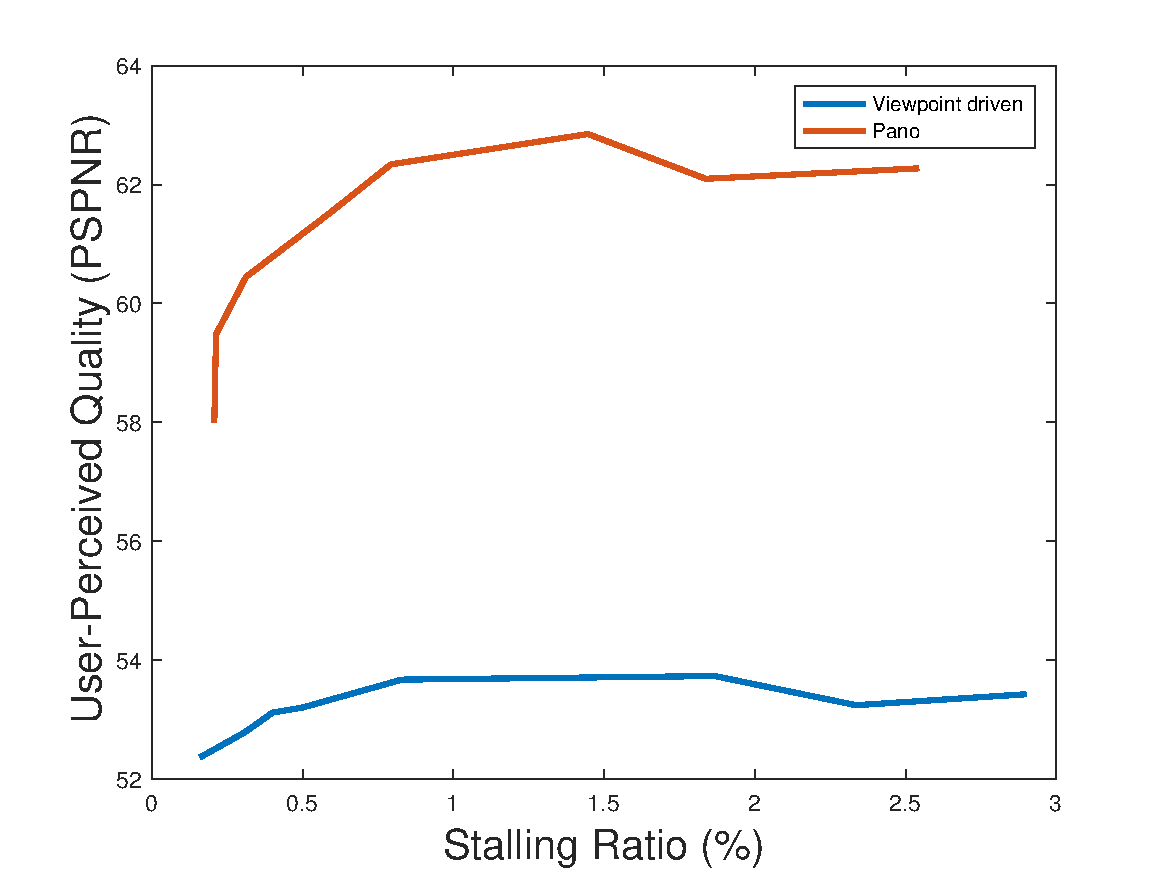
\includegraphics[width=3in]{images/intro-result.pdf}
  \caption{Performance of \name and the popular viewpoint-driven approach on \fillme \vrvideos and \fillme real-user viewpoint traces over an emulated link of \fillme($\pm$\fillme) Mbps.
  Full results are in \S\ref{sec:eval}.}
  \label{first_image}
\end{figure}

%\begin{figure}[t!]
%  \centering
%  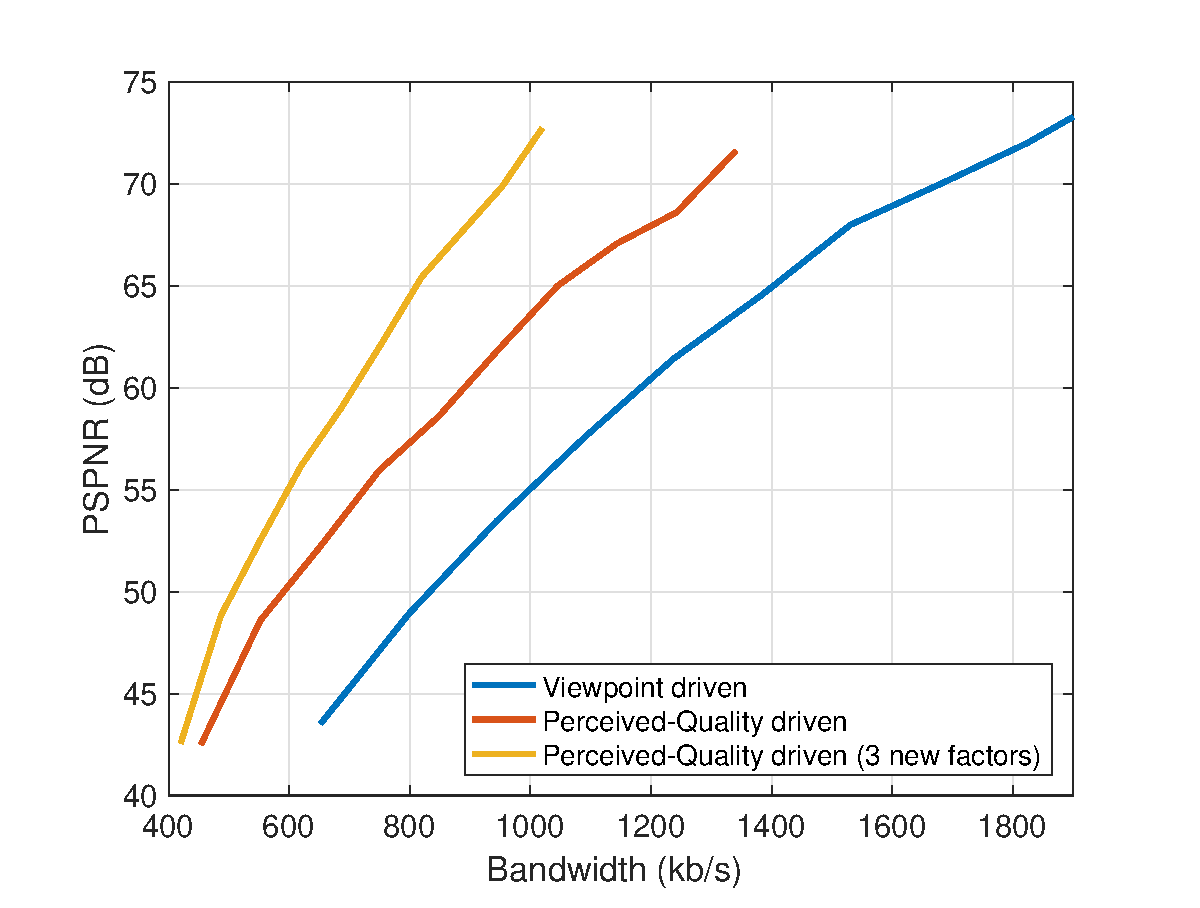
\includegraphics[width=2.5in]{images/improvement.eps}
%  \caption{Effectiveness of \name at reducing the bandwidth consumption and improving QoE. \jc{TODO. an example graph with two curves comparing \name and a canonical \vr video streaming protocol. }}
%  \label{fig:intro-improvement}
%  \end{figure}

The rationale behinds these opportunities is the fact that people have a limited span of attention.
For instance, as a viewer moves the viewpoint, it does increase the area that has to be streamed, but the viewer's ``per-pixel'' attention  (\ie sensitivity to quality distortion) drops as a result of having to spread the limited span of attention across a wider region.
We notice that similar ideas were explored in the context of video encoding with the concept of ``Just Noticeable Difference'' (JND)~\cite{??,??,??}---the minimal visual difference perceivable by humans, \eg viewers generally have larger JND when watching a more complex scene. 
However, conventional JND only models the content-level factors (it deals with static viewpoint), as opposed to the factors specific to the behaviors of \vr video viewers. 

This paper presents {\em \name}, an encoding and streaming system that optimizes the user-perceived QoE of \vr videos.
\name makes three contributions.

\vspace{0.1cm}
{\em First, \name presents a new QoE model that builds on the concept of JND to incorporate the new \vr video-specific factors (\S\ref{sec:jnd}).}
We ran an IRB-approved user study to quantify the impact of three factors---viewpoint velocity, relative depth-of-field, relative luminance---on viewer's sensitivity to quality degradation. 
In addition, we also take distance-to-viewpoint (commonly used in prior work) as a factor that affect the QoE.
We call the resulting JND model as {\em \vrjnd}. 
It can predict, for any given video and viewport trajectory, the minimal quality degradation likely be perceivable by the viewer.
An interesting empirical finding is that the new viewer-driven factors are largely independent to each other, which vastly simplifies the modeling of impact of multiple factors on JND, which would otherwise have to explore the space of an exponential number of combinations of multiple factors.
%Their likely independence might explained by \jc{what's the intuition here?}


\vspace{0.1cm}
{\em Second, \name proposes a novel spatial tiling mechanism to fully utilize the new JND model (\S\ref{sec:tiling}).}
To best utilize the proposed \vrjnd framework, the video encoding should allow different quality levels be applied to different regions in cognizant to the spatial distribution of \vrjnd values.
Unfortunately, we found the existing equal-sized square tiling (\eg 12$\times$6) often is far from ideal---a tile can be too coarse-grained (\ie unable to adapt the quality level according to \vrjnd) or too fine-grained (\ie low encoding efficiency).
%In fairness, the square tiling is designed to serve only one purpose of differentiating regions closer to the viewport center from the rest.

In contrast, \name splits the \vr video into square tiles of different sizes in order to roughly match the spatial boundaries of \vrjnd. 
Each tile is then encoded in multiple levels of quantization parameter, or QP, (like in prior work).
In some sense, this is a compromise between the more radical region-of-interest encoding (in which each object can be encoded differently) and the square tiling which simplifies the rendering of multiple tiles each with different QP levels.



\vspace{0.1cm}
{\em Finally, \name proposes an adaptive streaming protocol that is (a) robust to randomness of viewpoint movements, and (b) compatible with existing DASH protocols (\S\ref{sec:control}).}
At the first glance, allocating quality level based on user actions seems susceptible to randomness (\ie prediction errors) of the head movement. 
On the contrary, we show that it is possible to allocate quality level per tile in a way that tolerate substantial errors of viewpoint prediction. 
The reason stems from the fact that \vrjnd value of a region remains almost same for a range of actions (\eg \vrjnd remains the same as long as the viewpoint velocity is over a threshold), so what we need is to not to accurately predict the exact trajectory of the viewpoint, but rather the {\em range} of user actions.

Another practical challenge facing \name is that unlike traditional adaptive streaming, calculating \vrjnd requires real-time input from both the client (the real-time user trajectory) and the server (the pixel-level video content), making it incompatible to the mainstream DASH protocol which stream videos from stateless HTTP web servers. 
%on the server (\ie cannot be done by the client itself), so it is incompatible with the mainstream DASH protocols which stream videos from stateless HTTP web servers. 
%to determine the perceived quality of a chunk require some computation based on the video data on the server side, so in theory, it is incompatible with the mainstream DASH protocols which stream videos from stateless HTTP web servers.
%This is not a problem in non-\vr videos or existing \vr video protocols, because calculating the perceived quality of a chunk only depends on the available bandwidth and user viewport, both are locally accessible on the client side.
%However, the perceived quality in \vrjnd depends on the video content and user actions (\ie viewport trajectory and its projection), so the client cannot estimate the user-perceived quality without having the video content in the first place. 
%One approach to this conundrum is to let the video client upload the user action information to the server which then makes adaptation decisions, but this goes against DASH's HTTP-based architecture.
%Instead, in this work, we have taken a pragmatic stance to work within the constraints that have spurred the growth of video traffic---streaming videos from web servers over HTTP, like in DASH.
To run \name over the DASH protocol, we {\em decouple} the bitrate adaptation into an offline phase and an online phase.
In the offline phase, we pre-compute the best quality levels for only a few carefully picked possible values of the user action information (viewport trajectory and its projection), and send these estimates as part of the DASH metafile to the client at the beginning of a video session. 
%The basic idea is that it is possible to pre-compute the best quality levels for only a few carefully picked possible values of the user action information (viewport trajectory and its projection), and send these estimates as part of the DASH metafile to the client at the beginning of a video session. 
In the online phase, the client estimates the user action (as described above) and pick the quality level by the ``nearest neighbor'' among the user inputs that have been pre-computed. 
%The intuition behind pre-computing only a few user-action inputs is an empirical observation that in \vrjnd the impact of the user-action input is non-linear; \eg when the viewport movement speed is over some threshold, its impact on \vrjnd and the QP adaptation changes only marginally (probably because the viewer will be very insensitive).


\vspace{0.2cm}
We implemented a prototype of \name.
\jc{on what platform}
We ran a pilot study on one content provider with \fillme sessions. \jc{how many viewers? what types of videos?}

Our experiments show that \name can save 45\% bandwidth compared with state-of-art 360-video streaming solutions, without decrease of perceived quality.
\jc{add a line to describe the final user-rating based end-to-end experiments}



%!TEX root = main.tex

\section{Motivation}
\label{sec:motivate}

\begin{figure*}[t!]
  \centering
  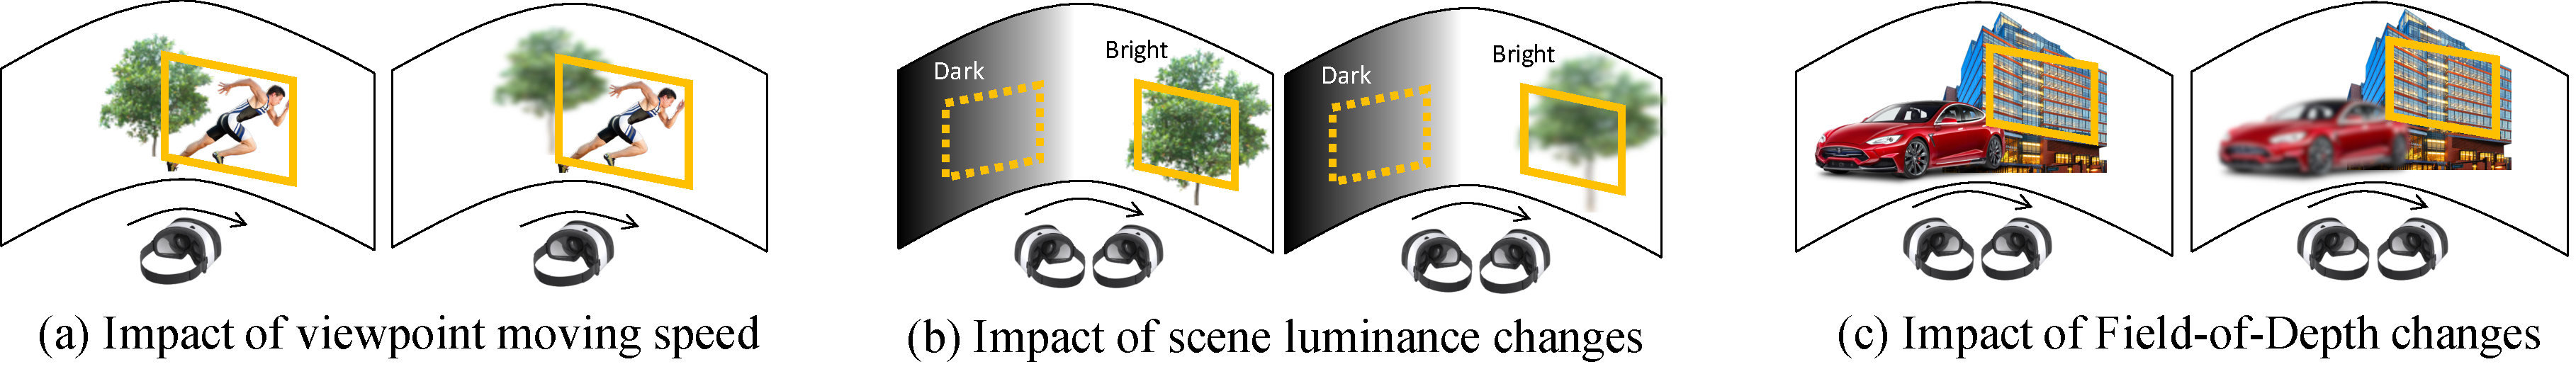
\includegraphics[width=0.9\textwidth]{figures/examples.pdf}
  \caption{Illustrative examples of the three \vr video-specific factor, and how they help save bandwidth by selectively reducing the quality of part of the video without affecting the user-perceived quality. The yellow boxes indicate the viewport (dashed ones are previous viewport). 
In each subgraph, the left-hand side and the right-hand side have similar perceived QoE, despite the quality distortions on some objects.}
  \label{fig:examples}
  \end{figure*}

We start with a background on \vrvideo streaming and today's common approach (\S\ref{subsec:background}, a full discussion on related work can be found in \S\ref{sec:related}).
Then, we outline several novel observations on user-perception of \vrvideo quality which inspire new opportunities to optimize the \vrvideo quality (\S\ref{subsec:opportunities}), and empiricially analyze their potential improvement for QoE (\S\ref{subsec:potentials}).
Finally, we highlight the challenges that must be addressed to unleash the potential benefits.


\subsection{Background of \vr video streaming}
\label{subsec:background}

%\mypara{\vr video streaming}
%\mypara{\vr videos coming to age}
%\vr video streaming is coming to age. 
By 2022, there will be over 55 million active VR headsets in the US, which is as many as paying Netflix members in the US in 2018~\cite{https://qz.com/1298512/vr-could-be-as-big-in-the-us-as-netflix-in-five-years-study-shows/}.
Almost all major content providers (YouTube~\cite{??}, Facebook~\cite{??}, Netflix~\cite{??}, Vimeo~\cite{??}, Amazon Prime~\cite{??}, Hulu~\cite{??}, iQIYI~\cite{??}, YouKu~\cite{??}) launched {\em streaming services for \vrvideos} on multiple  platforms~\cite{oculus,samsung,daydreams,etc}, believing that \vr videos are the future of story telling. 
\jc{add more concrete statistics on the popularity of VR}

%\mypara{Delivery architecture} 
The proliferation of the \vrvideo content and devices is also spurred by the highly efficient and scalable delivery architecture. 
Today, \vrvideos can be delivered to millions of concurrent viewers through commercial CDNs, in almost the same way non-\vr videos are delivered.
A \vrvideo is first encoded by a \vr encoder, which transcodes and chops the video into segments (or chunks); these video segments are then distributed to geo-distributed CDN edge servers; and finally, a client player (headset or smartphone) streams the video segments sequentially from the nearby CDN server using standard HTTP(S) (or DASH) protocols~\cite{hls,https://www.wowza.com/solutions/streaming-types/virtual-reality-and-360-degree-streaming}.
\jc{other than the client-side adaptation scheme, is there some fundamental diff or non-trivial steps involved in the preparation/dissemination of \vr content?}

To handle with last-mile bandwidth fluctuation, the video segments are encoded in multiple quality levels (usually quantization parameters or bitrates), and during playback, the \vrvideo player can switch quality level at the boundary between any two segments, in much the same way as non-\vr videos.
%Like non-\vr videos, \vrvideo streaming needs to cope with bandwidth fluctuation by adapting the quality level in order to strike a balance between video quality and bandwidth consumption.
%\mypara{Existing \vr video streaming protocols}
However, a distinctive feature of \vr video streaming is that the viewer's attention is {\em unevenly} distributed over a large area, with more attention centered around the viewport, whereas non-\vr videos are displayed on a fixed desktop or smartphone screen, os the unevenness of attention is less obvious.
Thus, \vrvideo streaming solutions also explore the {\em spatial} dimension: each video segment is spatially partitioned into tiles, each of which is encoded in multiple quality levels, so that different quality levels be used for different tiles depending on their {\em distance-to-viewport} ({\em DoV}), with higher quality in area closer to the user's viewpoint and lower quality for rest of the space.
This improves the perceived quality with the same or even less bandwidth consumption. 

%These {\em viewport-driven} protocols (\eg~\cite{??,??,??}) that the user-perceived quality of a spatial region is a function of the encoded quality and the region's distance to the viewport center.
Nevertheless, the gain of these {\em DoV-driven} protocols (\eg~\cite{??,??,??}) is limited, because the video segments must be short (typically one second, as opposed to 4-10 seconds in non-\vrvideos) so that the player can adapt the quality level as the viewpoint moves. \jc{add a concrete number for the size inflation due to the short chunk duration}
Despite many viewpoint-driven streaming~\cite{??,??,??} protocols or tiling mechanisms, this basic limit remains.



%\begin{figure}[t!]
%  \centering
%  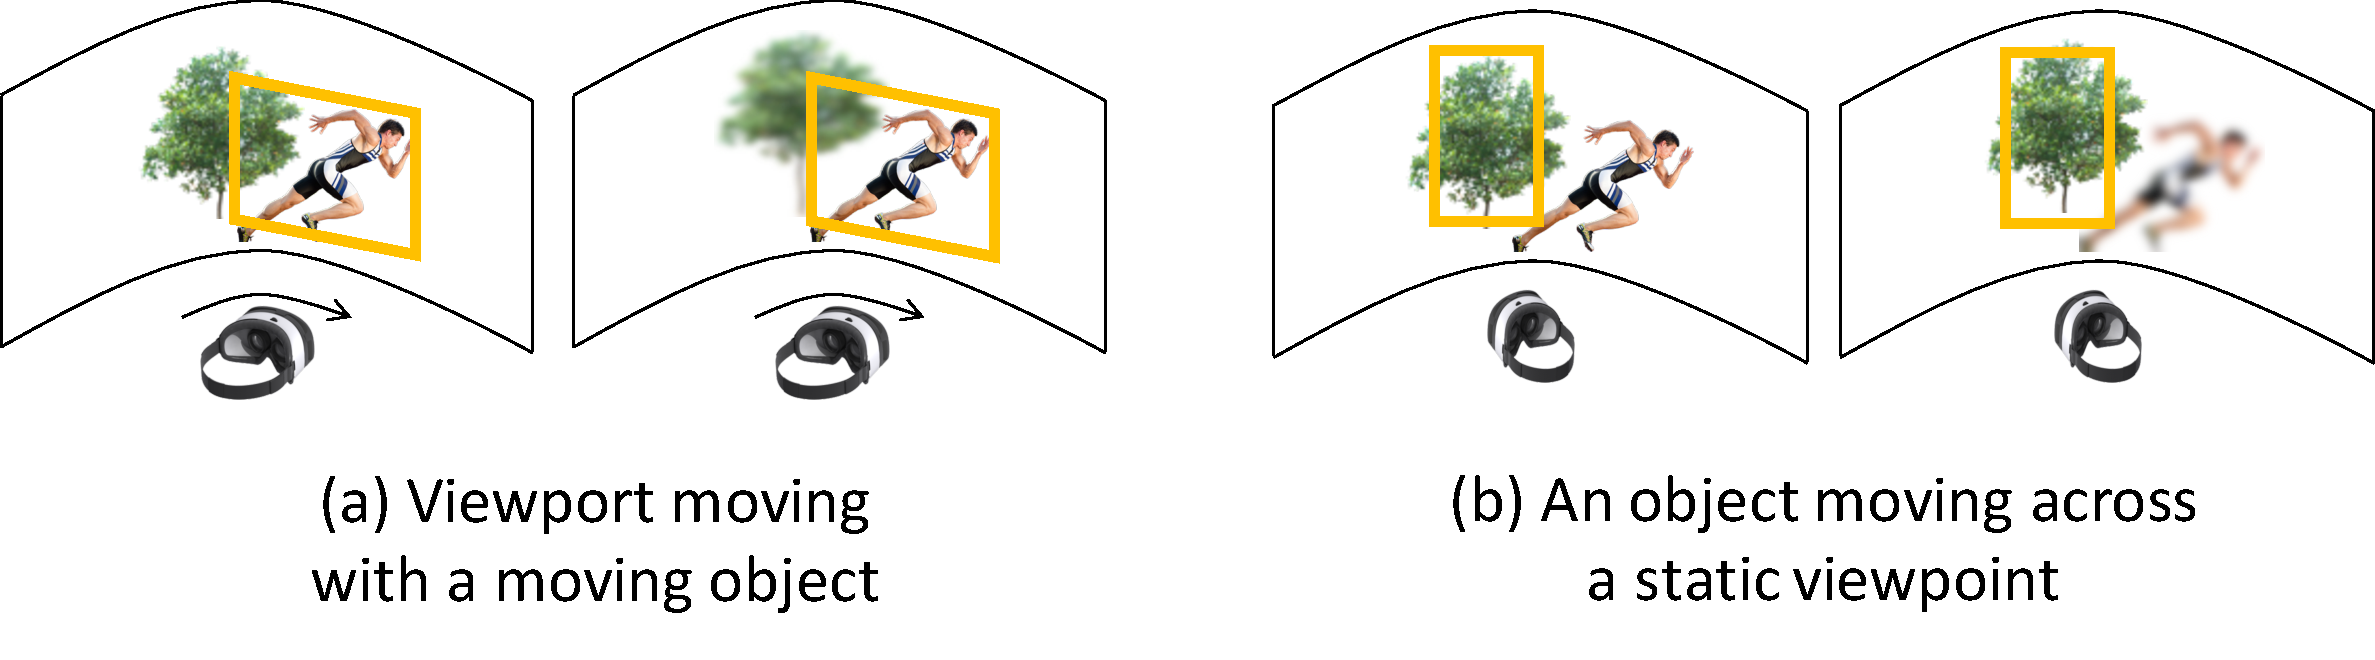
\includegraphics[width=0.5\textwidth]{figures/example-velocity.pdf}
%  \caption{Illustrative examples of the first \vr video-specific factor. 
%  Viewers tend to be insensitive to quality distortions of the objects moving at a high speed relative to the viewport, which can be (a) an object moving across a static viewport, or (b) the viewport moving across a static background. The yellow boxes indicate the viewport. 
%  In (a) and (b), the left-hand side and the right-hand side have similar perceived QoE, despite the quality distortions on some objects.}
%  \label{fig:example-velocity}
%  \end{figure}
%
%\begin{figure}[t!]
%  \centering
%  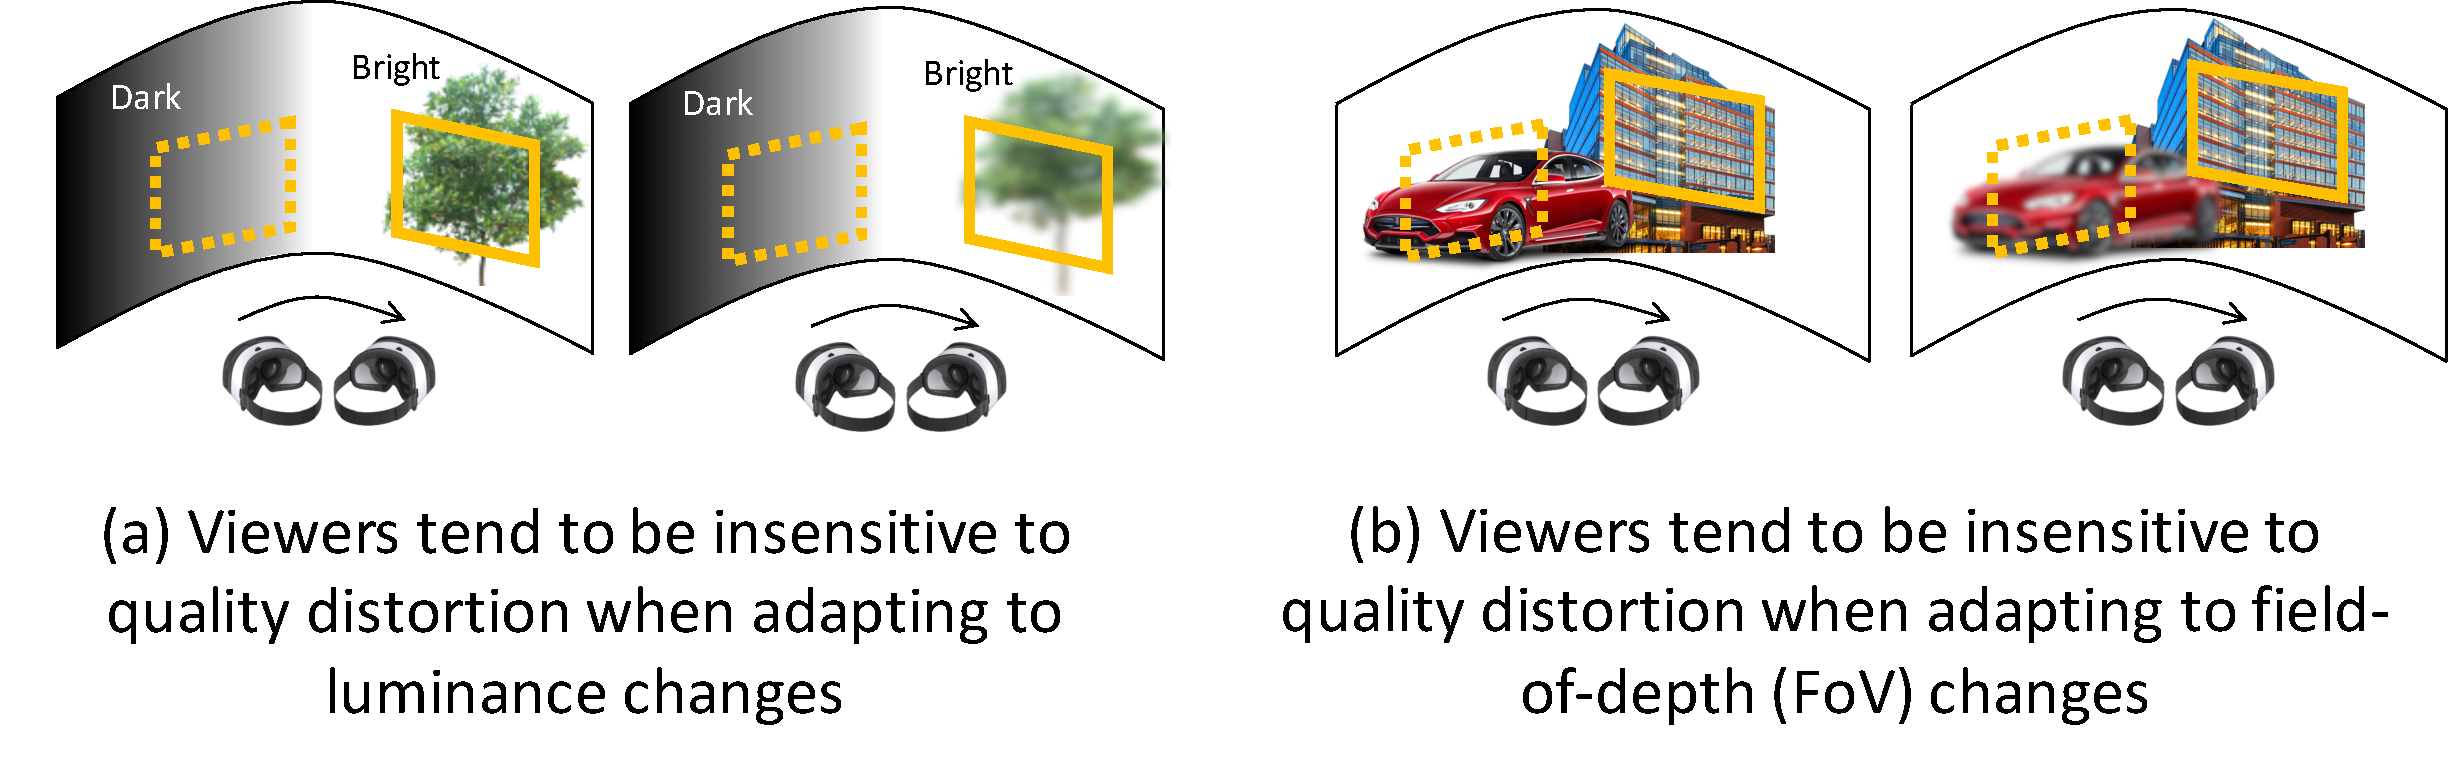
\includegraphics[width=0.5\textwidth]{figures/example-luminance-fov.pdf}
%  \caption{Illustrative examples of the 2nd and 3rd \vr video-specific factors. 
%  Viewers tend to be insensitive to quality distortions when (a) adapting to changes in luminance and when (b) an object has a different field-of-depth to the viewport.
%  The dashed boxes and solid boxes indicate where the viewport was and where it is now, respectively.
%  In both sub-figures, the left-hand side and the right-hand side have similar perceived QoE, despite the quality distortions on some objects.}
%  \label{fig:example-luminance}
%  \end{figure}

\subsection{New quality-determining factors}
\label{subsec:opportunities}

The driving intuition behind this work is that {\em through a deeper understanding of how viewers perceive \vrvideo quality, one can improve video quality or save bandwidth consumption without drop in perceived quality}.
Here, we briefly introduce three factors that can greatly affect the perceived quality of \vrvideos but have not been considered by existing \vrvideo streaming solutions. (\S\ref{sec:jnd} providers an in-depth analysis of these factors.)
%While the uneven distribution of the viewer's attention affects the QoE-bandwidth tradeoff, our first key observation is that it is just one of {\em several \vr video-specific factors that can heavily influence the perceived QoE of \vr videos but have yet to be fully explored}. 
%In particular, this paper examines the three following factors:

%\jc{need to visualize the three factors}

\begin{packeditemize}

%\myparashort
\item {\bf Factor\#1: Viewpoint moving speed.} 
%A key feature of \vr videos is that users can freely move their viewpoints. 
As the viewer moves her viewpoint, it also reduces the sensitivity to the quality distortion; and intuitively, the higher the speed, the lower the sensitivity. 
Figure~\ref{fig:examples}(a) gives an illustrative example of how this observation helps save bandwidth: when the viewer moves the viewpoint (\eg to track a moving object, as in the example), we found that reducing the quality level of static objects has little impact on user-perceived quality.
Similarly, when viewport is static, the viewer will tend to be insensitive to quality distortion of fast moving objects. 
%Consequently, as the viewers watch the video while moving their heads, they sometime report higher perceived quality than other static viewer perceive on the same video at the same objective quality level.
%the perceived quality is significantly improved, since user is unable to detect the distortion. 


%\myparashort
\item {\bf Factor\#2: Change in scene luminance.} 
Our second observation is that as the viewer moves her view around, the viewed region may switch between different levels of brightness, or luminance, and when the content changes from dark to bright (and vise versa), user's ability of detecting quality distortion also drops for a short period of time (typically \fillme seconds).
Figure~\ref{fig:examples}(b) illustrates a simple example of how one can carefully lower the quality level of part of the video without causing any drop in the user-perceived quality.
%When user wears a HMD in VR display, environmental brightness perceived by eyes is totally depended on luminance of video content itself.  
%As a result, when watching the same content encoded in the same objective quality, people report different levels of subjective quality depending on whether they have just watched something in different levels of luminance.


%\myparashort
\item {\bf Factor\#3: Differences in depth-of-field (DoF).} 
Our third observation is that a viewer can only be sensitive to the quality distortion of one of two objects, if they have different DoFs (\eg one being much closer to the viewer than the other).
Many \vr displays can precisely simulate the depths-of-field (DoF) by projecting an object to the two eyes with a specific binocular parallax (disparity) \jc{citation?}. 
Figure~\ref{fig:examples}(c) illustrates how one can reduce quality level of objects of different DoF than the object the viewer currently looks at\footnote{This paper assumes the object closest to the center of the viewport is the one watched by the viewer, which may not always hold. But this can be fixed if some gaze tracking mechanism (\eg~\cite{??,??}) is employed.}.
%We found that objects with small DoF (\ie closer to the viewer) have greater parallax, which lowers the viewer's sensitivity to quality distortion due to binocular fusion.
%As a result, a viewer might give different levels of attention to the objects of different DoF's, even if they are all close to the center of the viewport.

\end{packeditemize}
%\jc{why today's videos don't use them.}
We want to make two important remarks on these opportunities.

\myparaq{What is new about them}
While these factors (except DoF) have been studied in the context of traditional non-\vr videos, their benefits are greatly amplified in \vrvideo by the free viewpoint movements and the ability to track them. 
For instance, in non-\vr videos, fast-moving parts of the video may be given lower quality than static parts, but \vrvideos open up new opportunities as the viewer may actually look at the moving object, thus one can use lower quality for the whole background. 
On the other hand, these factors are certainly different to traditional viewpoint-driven streaming adaptation, which assumes the user-perceived quality only depends on the distance-to-viewpoint. 


\mypara{Intuitive explanation}
The key intuition behind all these opportunities is that {\em each viewer has a limited span of attention}.
With the new features of panoramic view and immersive experience, the video size grow dramatically, but the span of attention remains largely constant\footnote{The span of attention does grow as the \vr headset shows a bigger virtual screen, but this is a much smaller increase compared to the size inflation of the whole \vrvideo.}. 
Consequently, a viewer will give less attention to the specifics of a \vr video, which in turn reduces the sensitivity to the quality distortion at some parts of the video, creating a multitude of room for improving the bandwidth-QoE tradeoffs, including viewport-driven adaptation as well as the three aforementioned factors.


%\jc{
%\begin{itemize}
%\item p1: we first extend the jnd model with several \vr specific factors, 1, 2, 3
%\item p2: with the new jnd model (explained latter), the potential improvement is tremendous!
%\end{itemize}
%}




%The uneven distribution of \vr user's sensitivities can be explained by the attention theory~\cite{??,??}, which has been successfully applied to specialized video encoder and human-computer interface. 
%The key concept is the just-noticeable difference (JND)---a user tends to notice the difference between two images/videos, only after the difference is greater than a threshold of JND, which depends heavily on the image/video content (as well as the context of the viewer).
%\jc{add a few examples of JND, like content luminance, texture complexity}

%The existing viewport-driven streaming protocols can be seen as one design point of using JND which only depends on the distance between a region and the viewport center. 
%We have seen a few efforts to introduce the existing JND-based attention models in video streaming~\cite{??,??}, although so far their real application so far has been quite limited.


\subsection{Potential for improvement}
\label{subsec:potentials}

Next, we use a real-world dataset to analyze the potential practical QoE improvement and bandwidth savings of the new opportunities. 


\begin{table}[t]
\begin{tabular}{rc}
 \hline
Videos & \fillme \\ \hline
Original resolution & \fillme by \fillme \\ \hline
Duration & \fillme$\sim$\fillme minutes \\ \hline
Views per video & \fillme \\ \hline
\end{tabular}
\caption{Dataset summary}
\label{tab:dataset}
\end{table}


\mypara{Dataset}
The dataset consists of \fillme \vrvideos, each watched by \fillme users.
The video dataset was provided by \fillme\jc{what's the source?}, and can be found in \fillme \jc{is there a public source?}
Each video was played by a \fillme device~\cite{??}
The video content covers three major categories: sports (\fillme), movies (\fillme), theater (\fillme).
Table~\ref{tab:dataset} gives a summary of the dataset.

\myparaq{How prevalent are these factors}
We first measure the prevalence of these new factors. 
Figure~\ref{fig:prevalence} shows the distribution of viewpoint-moving speed, luminance changes in a small time window, and DoF differences among objects in the viewport (which will not be differentiated by existing techniques).
We can see that they all occur for a substantial fraction of times. 
For instance, for more than 30\% of time, the viewpoint is moving faster than 20~degree/s. 
To put it into perspective, this means 30\% of time, the viewers are unlikely to perceive a \fillme\% drop in quality of the static background content (as we will show in \S\ref{subsec:??}).
Similarly, \jc{a sentence on the other two graphs.}


%%According to our data analysis, more than \fillme\% time, user's viewpoint is moving faster than \fillme \textdegree/s. 
%One of the most highlighted feature of VR video is that users can freely move their viewpoints. According to our data analysis, more than 30\% viewpoints are moving faster than 20 deg/s. (Fig. \ref{CDFspeed}) 
%When human viewpoint is moving, visual acuity is decreased in 2 different conditions: (1) if user is tracking an object, visual acuity decreases smoothly with viewpoint moving speed increases. (2) If user is not tracking an object, visual acuity decreases dramatically with viewpoint moving speed increases. \cite{speed}
%\jc{can you visualize such findings, and also show some numbers about the other two factors?}

\begin{figure}
  \centering
  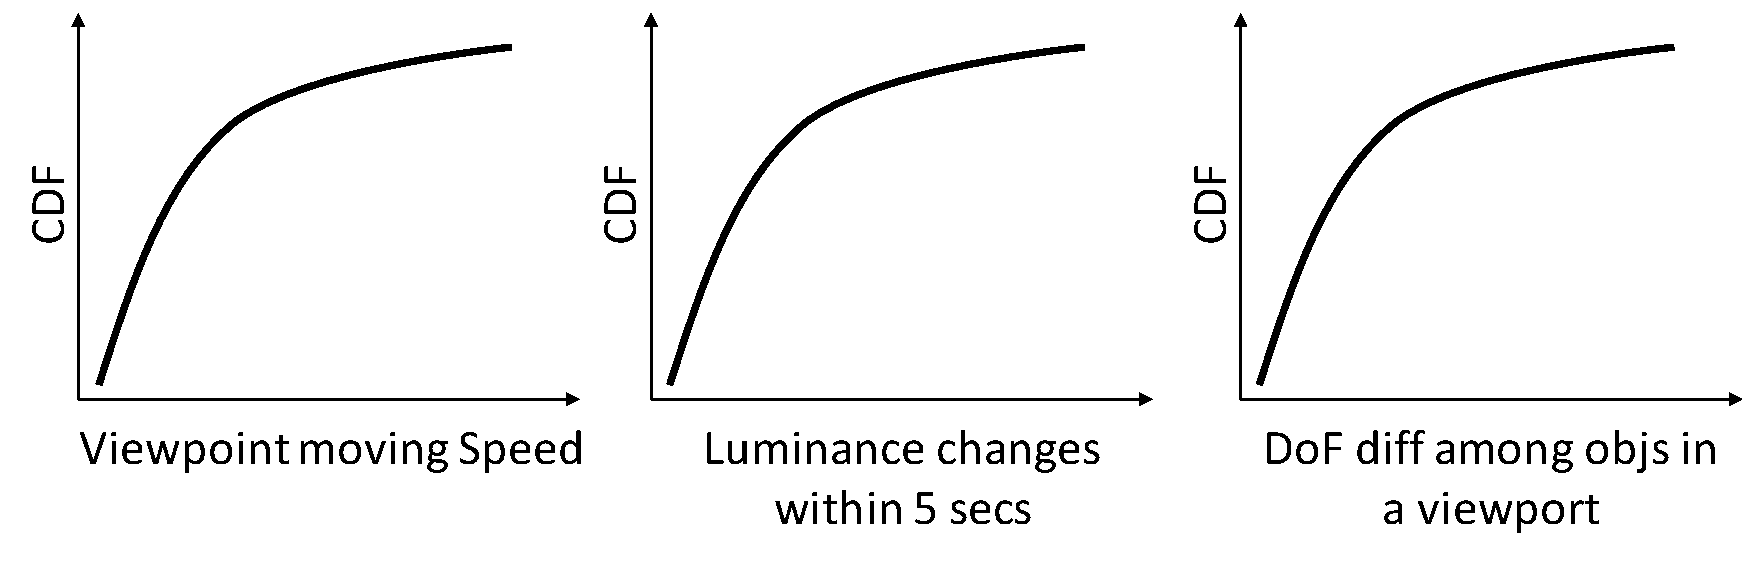
\includegraphics[width=0.5\textwidth]{figures/prevalence.pdf}
  \caption{Prevalence of the new opportunities.}
  \label{fig:prevalence}
 \end{figure}



\mypara{Potential gains in quality-bandwidth tradeoffs}
To show the practical benefits of these new factors in improving video quality, we consider an idealized scheme for encoding a \vrvideo, called {\em idealized \vrvideo}.
\jc{need details, how many quality levels? how many tiles? how to allocate quality levels under a given bandwidth?}
We compare it with a baseline inspired by the common DoV-driven approach: each frame is split into 
6*12 equal-sized rectangular tiles\footnote{\jc{how do we handle the problem of curved sphere? did we use any standard techniques?}}, and the tile covering the viewport are given the highest quality level, \jc{and how to allocate the rest tiles?}

Figure~\ref{fig:potential} shows that the idealized \vrvideo achieves a much better quality-bandwidth tradeoffs than the DoV-driven baseline.
We use peak signal-to-perceptible-noise ratio (PSPNR)~\cite{??} as an indicator of the perceived quality. 
We will discuss PSPNR in full details in \S\ref{sec:jnd}, but in short, it has a stronger linear correlation to subjective user rating than alternative measures (\eg PSNR).
The idealized \vrvideo can save \fillme\% bandwidth without drop in PSPNR, or improve PSPNR by \fillme\% (roughly an \fillme\% increase in user rating) using the same amount of bandwidth.

It should be noticed that both schemes are idealized since the viewpoint trajectory cannot be known in advance, but their comparison is indicative of the actual performance difference between the practical solutions. 

%Before giving the concrete design of an actual streaming protocol, we first present the potential for improvement of leveraging the \vr-specific factors. 
%To do so, we use a metric called PSPNR to denote the perceived quality of a viewer, which can be expressed by $F(P,P',A,v,d,\Delta d,l,\Delta l)$, where $P$ and $P'$ denote the original frame and the rendered frame respectively, $a=(x_a,y_a)$ the viewport center, $v$ the viewport moving speed, $d$ the DoF, $\Delta d$ the change in DoF, $l$ the luminance, and $\Delta l$ the change in luminance. 
%We will explain this metric in greater detail in the next section. 
%\jc{give a short description of how to understand PSPNR}

%PSPNR \cite{PSPNR} is applied as a metric to measure perceived quality. Real traces are collected from over 800 VR displays of 48 users. In our experiment, each video has 5 different bitrate level. We compare the performance of 3 methods:
%\begin{itemize}
%
%\item \emph{Viewpoint-driven VR streaming.} Video is cut into 6*12 spatial rectangular tiles. Tiles on user's viewpoint is allocated the high bitrate. For other tiles, bitrate is allocated linearly decreasing with its distance to user's viewpoint.
%
%\item \emph{Perceived quality driven VR streaming. (with 3 VR factors)} Suppose we can freely allocate bitrate to each spatial part of video without video tiling. Besides user viewpoint, content luminance and texture complexity, we also take consideration of viewpoint moving speed, content Depth-of-Field and light / dark adaptation, we do adaptive streaming to maximize user-perceived quality.
%
%\end{itemize}
%
%With consideration of content luminance and texture complexity, perceived-quality-driven VR streaming can save 30\% bandwidth compared with viewpoint-driven VR streaming providing the same PSPNR. Moreover, when we take consideration of viewpoint moving speed, object Depth-of-Field and light / dark adaptation, we can further save 20\% bandwidth.


\begin{figure}
  \centering
  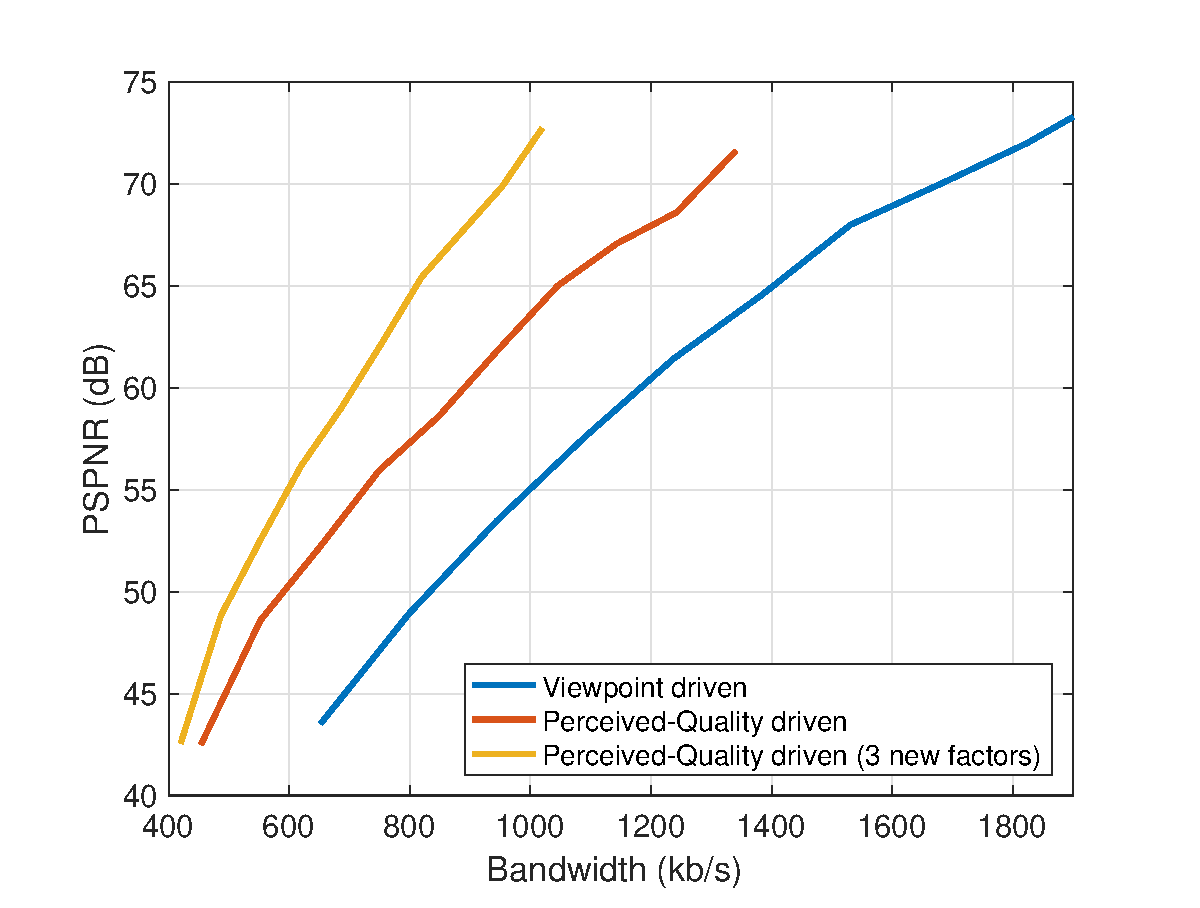
\includegraphics[width=2.5in]{images/improvement.eps}
  \caption{PSPNR-bandwidth tradeoff of (1) Viewpoint-driven VR streaming. (2) Perceived quality driven VR streaming. (3) Perceived quality driven VR streaming. (with 3 VR factors)}
  \label{fig:potential}
  \end{figure}




\subsection{Key challenges}

However, to fully explore these opportunities requires not only changing the quality objective function, but re-architecting several critical components of the video delivery pipeline. 
In particular, we identify three main challenges.

%In order to achieve perceived quality driven VR streaming, the core challenge is: perceived quality is related to both video content and user behavior, how to take together both-sides information to maximize the perceived quality. For specifically, there are three aspects:

\myparashort{Challenge 1: How to leverage the new quality-determining factors in \vrvideo streaming?}
%Challenge 1: Traditional Human Visual System (HVS) models can not measure perceived quality in VR video display.
Before designing the streaming protocol, we first need to incorporate the new quality-determining factors to how \vrvideo quality is measured. 
This, however, is not trivial, as most traditional video quality metrics focus on the impact of content-level dynamism (\eg users are relatively insensitive to quality distortion on a ``busy'' scene) while assuming the viewers are static.
On the contrary, the new quality-determining factors are driven mostly by user actions. 
So our first step is to incorporate them in existing video quality metrics.
%Perceived quality can be well-measured in traditional video display by building mathematical model from luminance, texture complexity and viewpoint-object distance to perceived quality. However, as we have mentioned, besides these existing factors, perceived quality in VR display is related to several new factors which are never modeled before. Their mathematical relationship to perceived quality, and how these new factors combined with existing factors together influence perceived quality are unknown problems.

\myparashort{Challenge 2: How should the \vrvideos be spatially tiled to fully exploit the new opportunities?}
%Challenge 2: Traditional grid-like video tiling scheme performs poorly in perceived quality optimization.
Second, the spatial tiling of \vrvideos must allow enough flexibility so that the quality adaptation logic can differentiate spatial regions to which the viewer has different sensitivity. 
For instance, it is ideal if the tiling is such that objects moving at different speed (\eg foreground vs background) can be assigned with different quality levels.
At a first glance, this can be done by using more fine-grained tiling, but this is not practical as finer-grained tiling will inevitably reduce video  coding efficiency and thus drastically inflate the bandwidth consumption.
Figure~\ref{fig:bitrate-efficiency} shows the average size inflation of all videos in the dataset (the tiled video size over the original video size), and that the size grows almost linearly with the number of tiles. 
So the existing equal-sized tiling mechanism is not sufficient to fully explore the new opportunities.

%To optimize perceived quality, we need to independently allocate bitrate of each spatial part of the video. Grid-like tiling scheme is a widely used method to solve the problem. Video is cut into several rectangular tiles with equal size which can be independently encoded / decoded. So we can allocate different bitrate to different tiles.
%
%However, traditional grid-like tiling performs poorly in perceived quality optimization in two aspects: 
%
%(1) Coarse-grained tiling causes coarse-grained rate allocation, and perceived quality obtained by coarse-grained rate allocation is far from that obtained by fine-grained rate allocation. We encode the video with different rate allocation granularity. We apply PSPNR to measure perceived quality and Fig. \ref{optimalencoding} shows the PSPNR-bandwidth tradeoff. Rate allocation with 3*6 / 6*12 granularity obtains -x\% / -x\% PSPNR compared with 12*24 granularity, this is a significant performance gap in perceived quality optimization.
%
%\begin{figure}
%  \centering
%  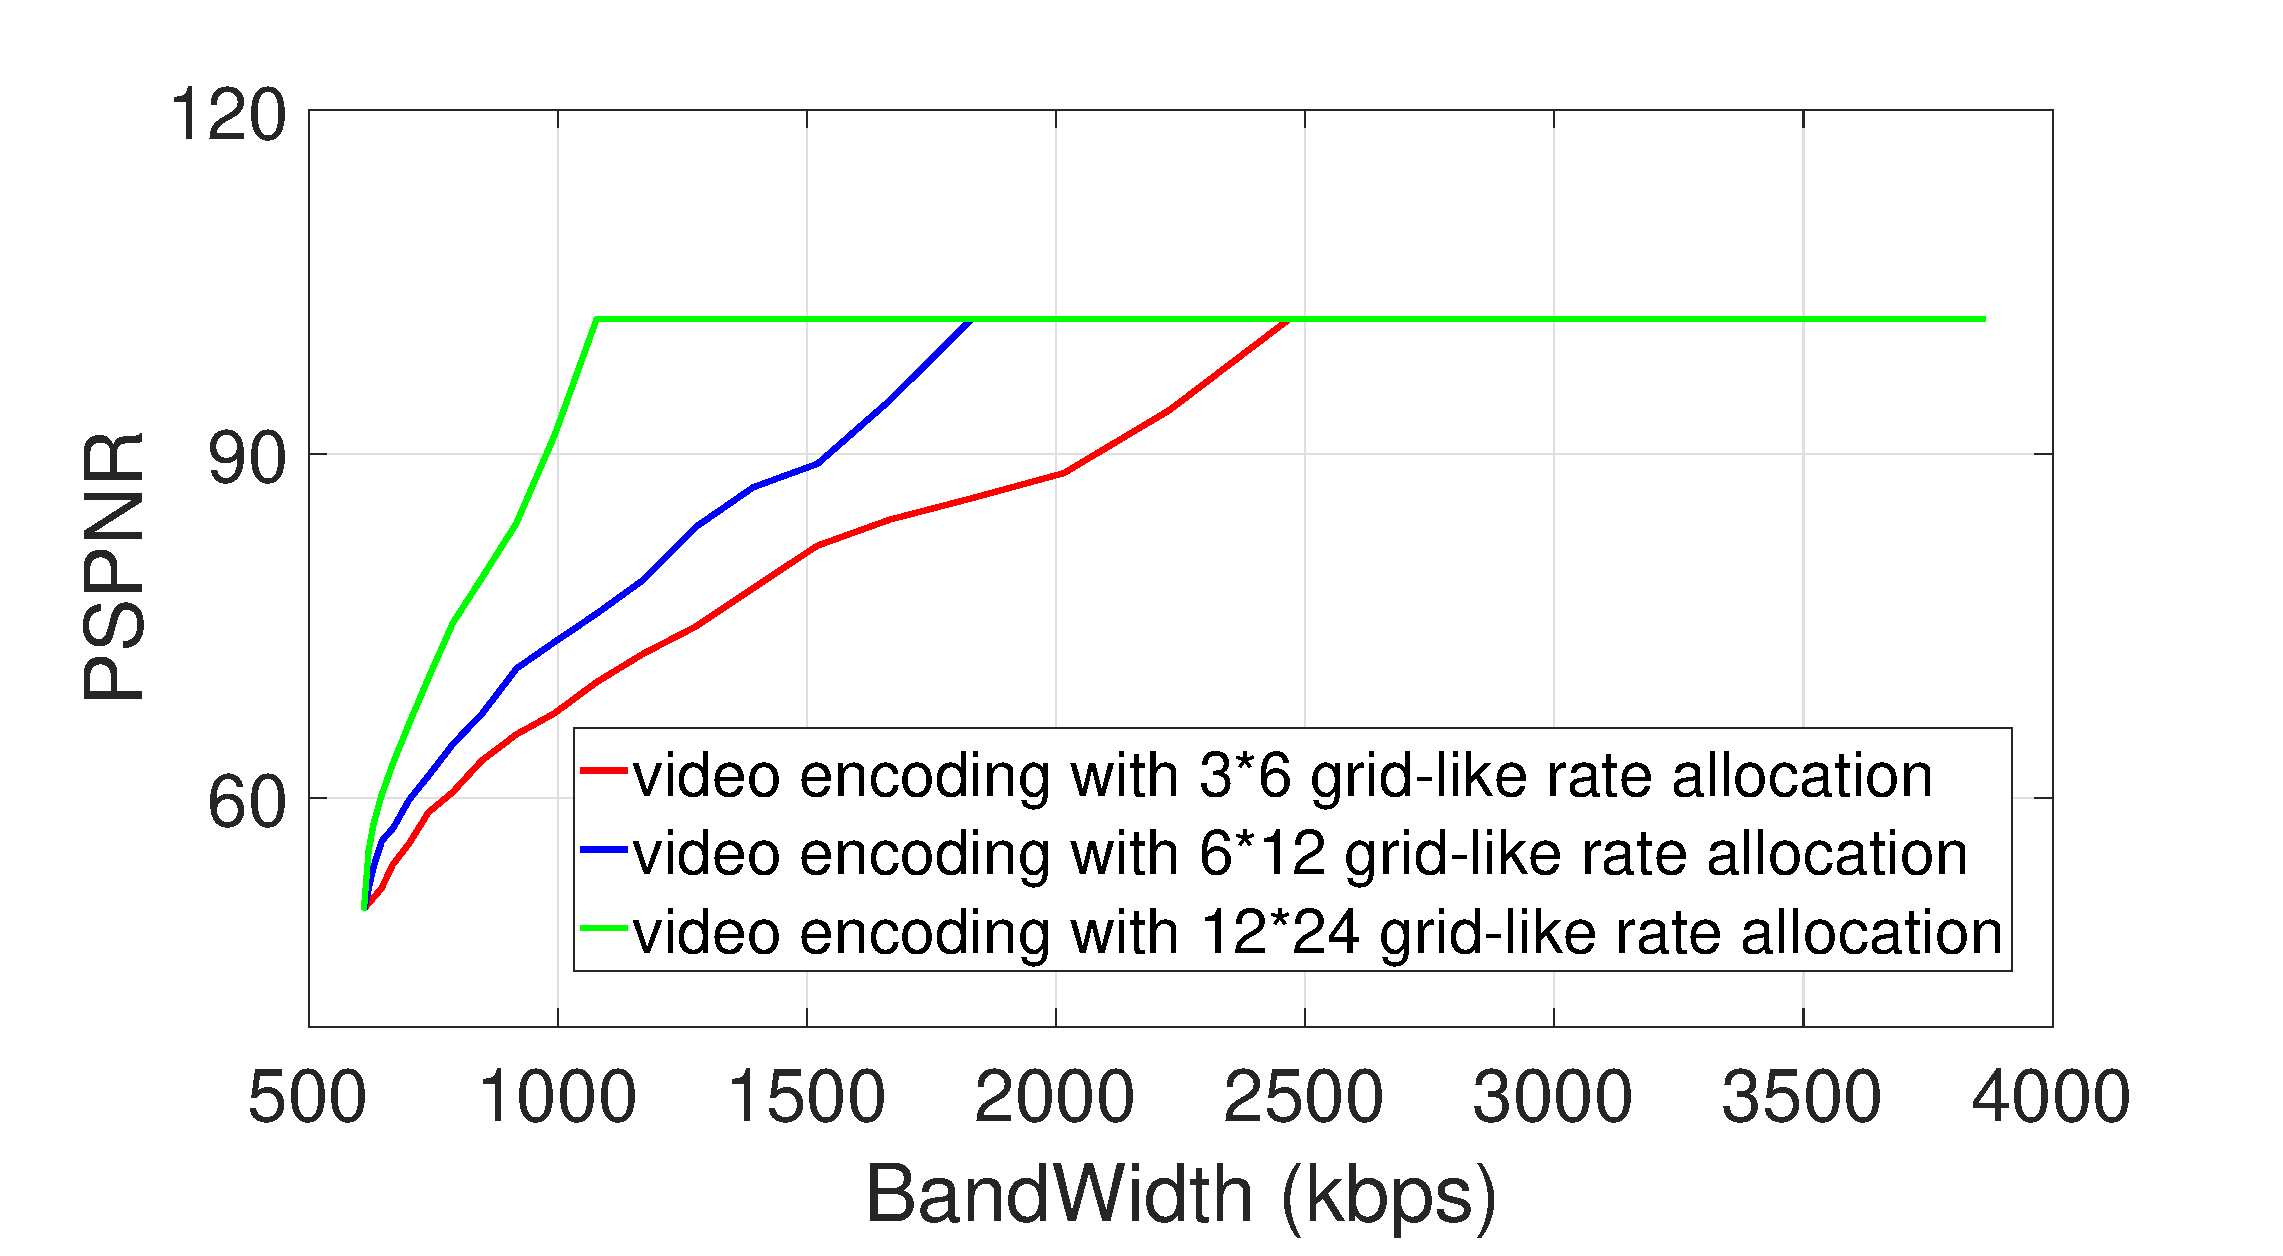
\includegraphics[width=2.5in]{images/optimalencoding.eps}
%  \caption{PSPNR-bandwidth tradeoff in video encoding with different granularity of rate allocation.}
%  \label{optimalencoding}
%  \end{figure}
%
%(2) Fine-grained tiling introduces serious bitrate efficiency problem in video encoding. In practice, each tile has to be encoded independently instead of encoded together. When we cut the video into tiles, the total video size is increased. Fig. \ref{bitrateefficiency} shows the video size of different tiling granularity compared with original video size. We find that cutting a video into 12*24 tiles introduces 50\% to 330\% additional video size compared to original video. This significantly lower its practical performance in perceived quality optimization, especially in low bandwidth situations where the bitrate efficiency problem is very serious.

\begin{figure}
  \centering
  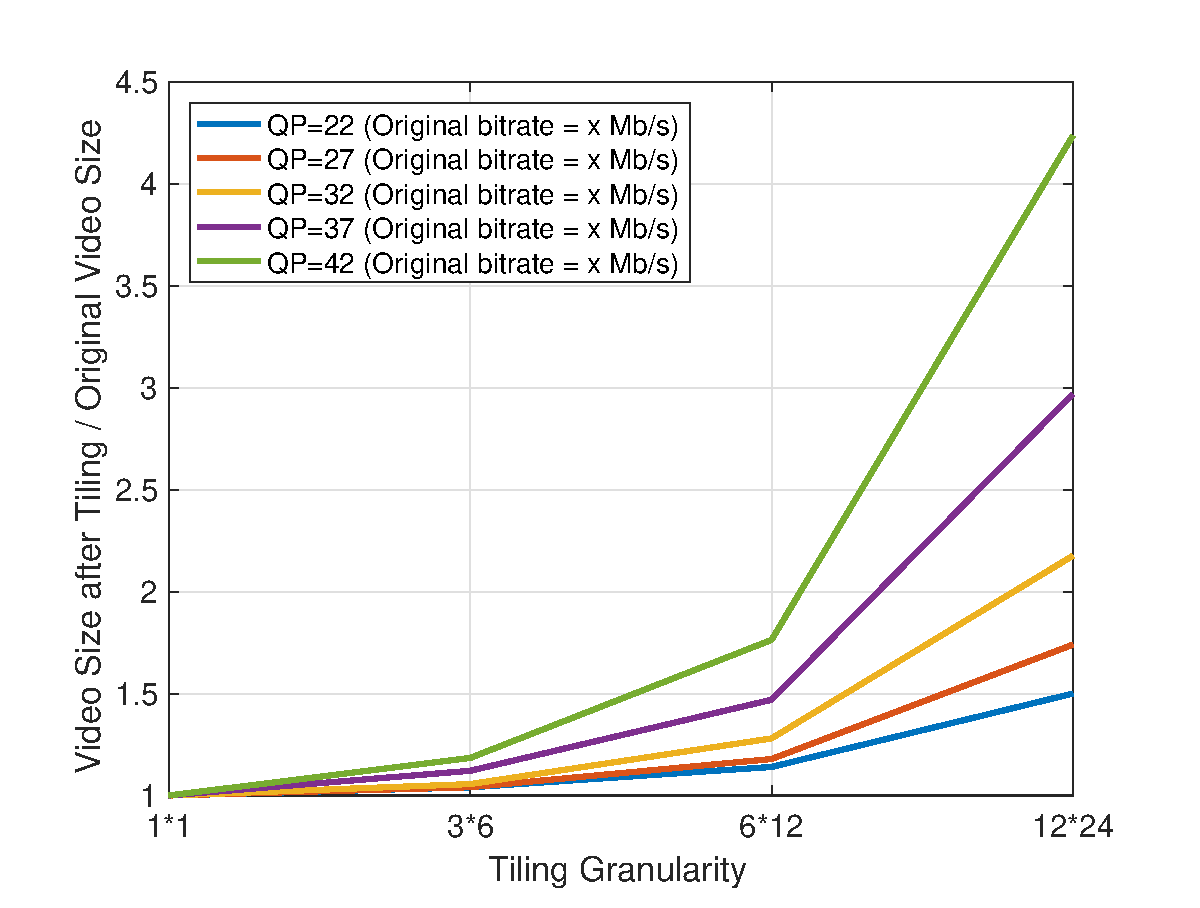
\includegraphics[width=2.5in]{images/bitrateefficiency.eps}
  \caption{The ratio of video size after tiling and original video size in each tiling granularity and each bitrate level. We notice that fine-grained tiling introduces serious bitrate efficiency problem, especially in low bandwidth situations in which the overall bitrate of each tile is low. \jc{pick one line. no need for five lines}}
  \label{fig:bitrate-efficiency}
  \end{figure}

\myparashort{Challenge 3: How to design a streaming protocol that is robust to noises in user action and compatible with the existing delivery infrastructure?}
%Challenge 3: Information needed for perceived quality computation is disparted on server-side and client-side.
Finally, the new quality-determining factors call for a revisit on the streaming protocol. 
On one hand, it seems the protocol must be sufficiently adaptive to cope not just fluctuation in bandwidth variation and viewpoint movement, but also real-time changes of the movement velocity, the scene luminance, and the depth-of-field. 
On the other hand, the streaming protocol must also be architecturally compatible with the HTTP-based delivery infrastructure that has spurred the rise of \vrvideos, so the quality adaptation is driven solely by the client (while the server passively server the video as web objects). 
Unfortunately, this is difficult because, as we will see, to calculate the optimal quality level, the client needs the knowledge of the video content before streaming the content. 

%To optimize perceived quality, client needs to compute the perceived quality of each bitrate allocation and then make decision. However, different from video quality which only related to video content itself, perceived quality depends on both video content and user behavior. Information of video content is located on server-side while information of user behavior is located on client-side. To get information of video content with current DASH, client has to pre-request in information of each pixel from server. This communication overload even exceed the overload of actual video streaming.





%!TEX root = main.tex

\section{\name overivew}

Next, we present {\em \name}, an end-to-end solution to the three aforementioned challenges.
As depicted in Figure~\ref{fig:overview}, \name modifies the three components of the video delivery pipeline. 
Before diving into the details of each component, we first give an overview of the rationale behind how they address the challenges, and put them in the perspective of existing video delivery pipelines. 



\mypara{Quality metric (\S\ref{sec:jnd})}
Building on a standard framework of video quality metric framework, we found the minimal changes needed to incorporate the new quality-determining factors (Challenge \#1) is to quantify their joint impact on the {\em minimal noticeable quality distortion}.
In other words, rather than building a \vrvideo quality metrics from scratch, one only needs to quantify the minimal noticeable quality distortion (\ie the lowest acceptable quality level) under any given viepoint-moving speed, change of luminance, and DoF difference. 
Moreover, our empirical analysis based on an IRB-approved user study reveals that the impact of these new factors on quality is largely mutually independent, which further reduces the efforts to profile the joint impact of these factors on \vrvideo quality.

\mypara{Offline tiling (\S\ref{sec:tiling})}
Unlike traditional tiling schemes which always split a video into same-size grids, \name splits it into {\em variable-size} tiles, with the tile boundaries roughly where the object moving speed, luminance, or DoF changes (illustrated in Figure~\ref{fig:tiling}). 
Each tile is then encoded in multiple levels of quantization parameter (QP). %, so that the quality level can be picked to optimize the perceived quality during playback time.
The key here is that \name allows regions with different sensitivity to quality distortion can be treated differently, while maintaining the same tiling granularity as traditional equal-size grid tiling, thus providing the necessary flexibility without exploding the bandwidth consumption (Challenge \#2).


\mypara{Online adaptation (\S\ref{sec:control})}
Lastly, we found that the new quality-determining factors have a non-linear impact on how video quality is perceived by users, which suggest that, rather than predicting the precise user action (\eg viewpoint position), it is sufficient to predict their {\em lower bound}, which helps tolerate the occasional prediction error of user action during playback (Challenge \#3).
Moreover, to enable client-driven adaptation, \name encodes a look-up table in the DASH manifest file so that the client can approximately estimate the perceived quality under different quality levels without access to the actual video content, thus compatible with today's video delivery architecture (Challenge \#3).


A final remark is that \name can be completely deployed by the content provider (who controls the video encoding) and client-side device (usually also managed by the content provider), with no change to the CDN infrastructure or the underlying HTTP streaming protocol, so it enjoys the same performance and authentication benefits as existing videos.


\begin{figure}
  \centering
  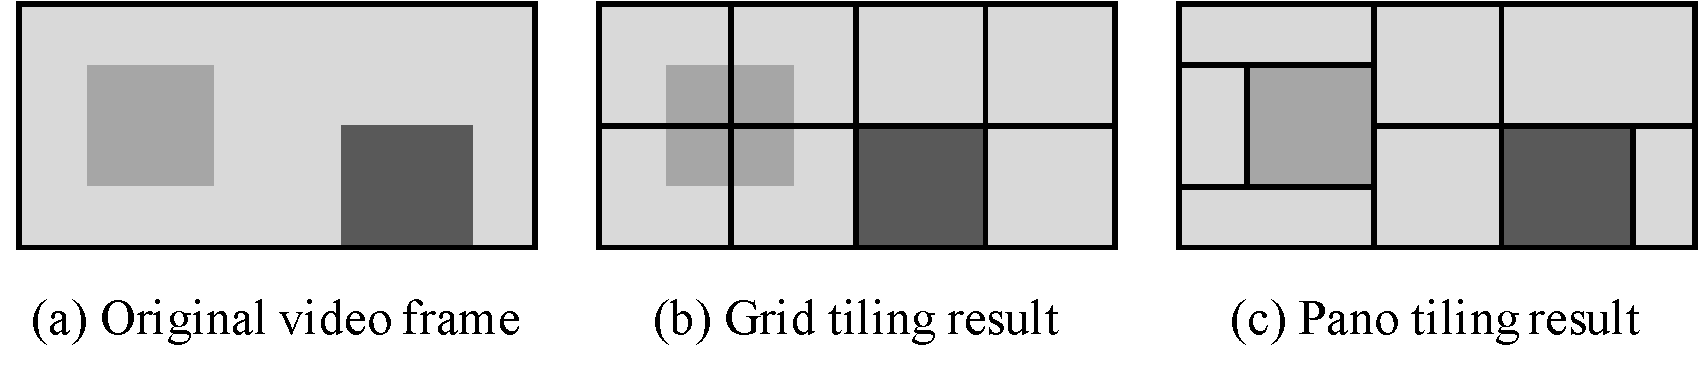
\includegraphics[width=0.5\textwidth]{figures/tiling.pdf}
  \caption{Illustrative example of \name tiling and traditional tiling. Each shade denotes a region with similar object moving speed, luminance, and DoF.}
  \label{fig:tiling}
 \end{figure}




%As stated in previous section, the biggest challenge of optimizing user-perceived quality is that perceived quality is related to both video content and user behavior. To solve the challenge, we show that perceived quality optimization can be decoupled: we can optimize video-content-related factors on server-side and optimize user-behavior-related factors on client-side.
%
%
%%\subsection{Insights}
%In this section, we show that in VR streaming, each visual factor influences user-perceived quality independently. So we can decouple them into several single factors to measure perceived quality respectively, then we design an server-side offline tiling scheme only with consideration of video content, and design a client-side bitrate allocation method only with consideration of user behavior.
%
%\textbf{Insight 1: Perceived quality model in VR display can be built by simply adding several new factors on traditional perceived quality model.}
%
%In traditional video display, there are many factors which influence user-perceived quality. Prior works have studied how single factors influence user-perceived quality. Moreover, \cite{distance} proves that, in perceived quality computation, several factors (luminance, texture complexity, etc.) can be considered independently. As a result, we can independently measure the influence of each factor as a coefficient, and multiply them together to obtain the final user-perceived quality.
%
%However, in VR display, there are some new factors which are never considered in traditional video display. So how these new factors, together with factors in traditional video display, influence the perceived quality in VR streaming, is an unknown problem. We intend to assume that they can also be computed independently, and then multiplied as coefficients together with traditional factors to obtain final user-perceived quality.
%
%To prove our guess, we set up a user study to evaluate how perceived quality is influenced by multiple factors. (Sec. 4) Our result shows that perceived quality model in VR display can be decoupled. We only need to simply add new factors to traditional perceived quality model.
%
%\textbf{Insight 2: Video tiling strategy can be optimized on server side.}
%
%In traditional grid-like video tiling scheme, video is cut into m*n rectangular tiles with equal size. 
%
%This tiling strategy has an obvious drawback: at most times the boundary between objects are not exactly on the boundary between two adjacent tiles. Fig. \ref{fig_insight_tiling} shows an example. In the video frame, there are two objects (Object A, Object B) and a background. In coarse-grained tiling (Fig. \ref{fig_insight_tiling}(b)), the object can not be exactly caught by one or several tiles. It leads to bitrate allocation of low performance. In fine-grained tiling (Fig. \ref{fig_insight_tiling}(c)), although the object can be caught by several tiles, it cut the video into too many tiles and many cutting lines are unnecessary. It leads to serious bandwidth efficiency problem as described in Sec. 2.3.
%
%
%\begin{figure*}[!t]  
%\begin{tabular}{cccc}  
%\begin{minipage}[t]{0.24\linewidth}  
% 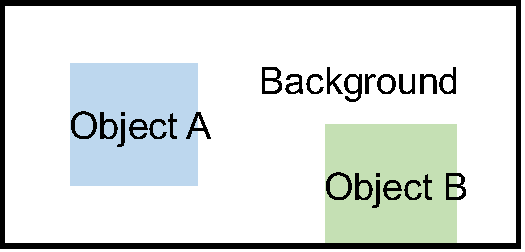
\includegraphics[width = 1\linewidth]{images/insight_tiling1.pdf}  
%     \center{(a) A video frame.}
%     \label{fig_insight_tilinga}
%\end{minipage}  
%\begin{minipage}[t]{0.24\linewidth}  
%    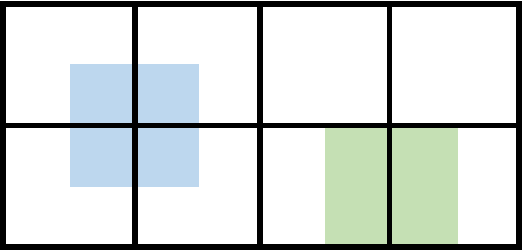
\includegraphics[width = 1\linewidth]{images/insight_tiling2.pdf}  
%     \center{(b) Grid-like tiling in coarse granularity.}
%     \label{fig_insight_tilingb}
%\end{minipage}  
%\begin{minipage}[t]{0.24\linewidth}  
% 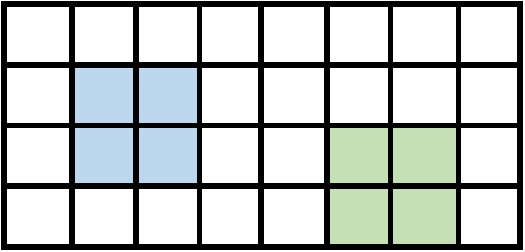
\includegraphics[width = 1\linewidth]{images/insight_tiling3.pdf}  
%     \center{(c) Grid-like tiling in fine granularity.}
%     \label{fig_insight_tilingc}
%\end{minipage}  
%\begin{minipage}[t]{0.24\linewidth}  
% 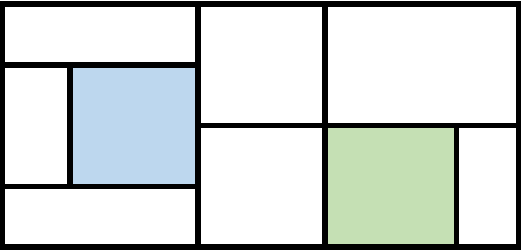
\includegraphics[width = 1\linewidth]{images/insight_tiling4.pdf}  
%     \center{(d) Object-based tiling.}
%     \label{fig_insight_tilingd}
%\end{minipage}  
%\end{tabular}  
%  \caption{An example of traditional grid-like tiling and object-based tiling.}  
%\label{fig_insight_tiling}
%\end{figure*}  
%
%Suppose we can know information about video content, we can cut the video based on objects like Fig. \ref{fig_insight_tiling}(d). In this method, we can obtain similar tiling granularity as Fig. \ref{fig_insight_tiling}(c) but remain similar tile numbers as Fig. \ref{fig_insight_tiling}(b). We think tiling scheme like Fig. \ref{fig_insight_tiling}(d) can outperform traditional grid-like tiling scheme. Moreover, since information of objects is only related to video content, it is totally independent from user. So object-based tiling can be completed offline on server-side.
%
%\textbf{Insight 3: Perceived quality computation can be decoupled.}
%
%Although accurately computing perceived quality needs the information of both video content and actual user behavior, we can precompute perceived quality of given video content with each possible user behavior situations on server-side, without any information of actual user behavior, and transform the computation result to client. Client only needs to choose the situation which match actual user behavior most, then uses given perceived quality value to approximate the actual perceived quality. Experimental results prove that we can obtain very good approximation accuracy with very little end-to-end exchanging overhead of computation result transforming. 
%
%
%\jc{need to mention \name is readily deployable. only changes the client-side and encoding, without involving the video sources and CDN operations}
%
%
%
%%\subsection{Key ideas to solve the challenges}
%%
%%Based on above insights, we decouple the visual characteristics due to video content and user viewpoint, and design a perceived quality driven VR streaming system which consider visual characteristics of video objects completely on server-side, and considers visual characteristics of user behavior completely on client-side. Specifically, we build our system based on following ideas:
%%
%%\begin{itemize}
%%
%%\item \emph{Measuring perceived quality in VR streaming by incrementally adding some new coefficients into traditional non-VR perceived quality model.} (\S 4)
%%
%%\item \emph{Server-side offline video tiling only based on of video content.} (\S 5)
%%
%%\item \emph{Server-side perceived quality precomputation and client-side approximation \& optimization.} (\S 6)
%%
%%\end{itemize}
%
%
%
%
%
%


%!TEX root = main.tex

\section{Quality model of \name}
\label{sec:jnd}

We start with the quality model of \name, which estimates the subjective user experience for a given video content and real-time user action (viewpoint position and velocity).
%We begin with a brief introduction of the traditional video quality metric framework on which we build our model and how the new quality-determining factors can be incorporated (\S\ref{subsec:jnd:framework}), and then provide detailed empirical analysis on the impact of these new factors affect the perceived quality (\S\ref{subsec:jnd:details}).

\subsection{A general video quality framework}
\label{subsec:jnd:framework}

%\jc{need to tighten the text}

%It is defined based on Just-Noticeable-Distortion (JND) theory \cite{JND}. Given the original video frame and a compressed video frame, user can notice their difference only if the difference between them is above a visibility threshold. When the different is under this threshold, it will not detected by user. This threshold is called Just-Noticeable-Distortion.
%
%Based on JND theory, PSPNR is defined by accumulating error of each pixel which can be detected by user:

We first briefly introduce the framework on which we build our video quality metric that incorporates the new quality-determining factors. 
We use Peak Signal-to-Perceptible-Noise Ratio (PSPNR)~\cite{PSPNR}, a widely-used metric to measure perceived quality. 
It improves on the classic Peak Signal-to-Noise Ratio (PSNR) by taking into account only the changes perceptible by the viewer.
So images with the same level pixel-level quality distortion (\ie same PSNR) can have different PSPNR values, if users tend to be less sensitive to one image (\eg typically more complex or darker, etc) than another.

The key to PSPNR is the notion called Just-Noticeable Difference (JND)~\cite{??}, which is the minimal changes in pixel value that can be noticed by viewers. 
PSPNR can be expressed mathematically as following
\vspace{-0.3cm}
\begin{alignat}{2}\
\label{f1} PSPNR = 20 \times \log_{10}\frac{255}{\sqrt{PMSE}}
\end{alignat}
\vspace{-0.3cm}
\begin{alignat}{2}\
PMSE=\frac{1}{MN}\sum_{x,y}\left[ |p_{x,y} - \hat{p}_{x,y}| - JND_{x,y}\right]^2 \times \Delta (x, y)
\end{alignat}
\vspace{-0.3cm}
\begin{alignat}{2}\
\Delta (x, y) =\left\{
\begin{aligned}
1, & &|p_{x,y} - \hat{p}_{x,y}| > JND_{x,y} \\
0, & &|p_{x,y} - \hat{p}_{x,y}| \le JND_{x,y}
\end{aligned}
\right.
\end{alignat}
where $M,N$ denote the image size, $p_{x,y}$ and $\hat{p}_{x,y}$ pixel values at $(x, y)$ in original video frame and compressed video frame, and $JND_{x,y}$ the JND threshold at pixel $(x, y)$.

PSPNR helps to model the user-perceived quality of \vrvideos, because it wraps all factors other than pixel-level distortion in the abstraction of JND, effectively {\em separating} the their impact on the perceived quality from the impact of of pixel-level distortion. 
Traditionally, the notion of JND has been shown to be related to a series of factors: texture complexity~\cite{??}, content luminance~\cite{??}, viewpoint-object distance~\cite{??} and so forth.
Following this approach, we empirically found that it is possible to incorporate the three new quality-determining factors in the calculation of JND.



%Compared with PSNR (which is widely used in evaluating video / image quality), the core difference of PSPNR is introducing a term $JND(x, y)$ for each pixel $(x, y)$. So how to compute JND for each pixel $(x, y)$ is an important issue. We will present our JND computation in the following section.
%
%The just-noticeable distortion (JND) provides cues for measuring the visibility of the Human Vision System (HVS). JND refers to the maximum distortion which cannot be perceived by human. It describes the perceptual redundancy of the picture by providing the visibility threshold. The JND model generally exploits the visibility of the minimally perceptible distortion.
%
%JND has been well-studied in traditional video display since 1995. The most basic and solid research is about the relationship between content luminance and JND. \cite{luminance1}  and \cite{PSPNR} prove that content with moderate content luminance have low JND value, while content with very high or very low content luminance have high JND value. 

%In recent years, based on the insight of content luminance - JND relationship, researchers have explored some more factors which are also related to JND, such as texture complexity, viewpoint-object distance (\cite{PSPNR}, \cite{distance}) and some other factors. Although the relationship between multiple JND factors may be complex, for simplicity, we can decouple them into several single factors. For example, \cite{distance} set up a user study to test the JND value with the combined effect of content luminance and viewpoint-object distance. The result proves that viewpoint-object distance can be considered independently from content luminance. It can be regarded as a coefficient which can be directly multiplied on JND value computed by content luminance. Based on this insight, JND computation for multiple factors is decoupled into several single factors. This significantly simplify the JND computation.

%\subsection{JND for \vr videos}

%
%
%In VR display, user experience is very different because 3 new factors should be taken into consideration: (1) viewpoint moving decreases visual acuity, (2) low Depth-of-Field decreases visual acuity and (3) light / dark adaptation decreases visual acuity. So previous JND model for traditional video display can not be directly applied on VR video display. Moreover, it is unknown that (1) how these new factors influence JND with combined effect of old factors, and (2) if they can also be decoupled into several single factors, like viewpoint-object distance \cite{distance}.
%
%Strictly answering these 2 questions needs to test JND value for each possible combinations of all factors (including all possible luminance, texture, viewpoint-object distance, viewpoint moving speed, Depth-of-Field and light / dark adaptation, which make up a 6-dimension feature space), which is not practical for a real-world user study. For simplicity, we imitate the user study in \cite{distance}, which makes only 2 factors variable and other 4 factors fixed, then we can know how is the combined effect of the 2 factors to JND, and if they can be decoupled to 2 single factors which independently influence JND.
%
%So we present 3 user studies: (1) JND v.s. luminance \& viewpoint moving speed. (2) JND v.s. luminance \& depth of field. (3) JND v.s. luminance \& light / dark adaptation. We evaluate the effect of 3 VR-only factors to JND, each with combined effect of luminance, since luminance is the most well-studied JND factor.
%
%We conduct the user study using real Head Mounted Device (HMD). Parameters of proposed HMD are listed as Table \ref{table1}:
%
%\begin{table}[h]
%\centering
%\caption{HMD Parameters}\label{table1}
%\begin{tabular}{|p{3.5cm}|p{3.5cm}|}
%\hline
%Equipment & Oculus GO\\
%CPU & Xiaolong 821 customized drive Edition\\
%Memory & 3GB\\
%Screen Resolution & 2560 $\times$ 1440\\
%Refresh Rate & 72Hz\\
%Fixed pupil distance & 63.5mm\\
%\hline
%\end{tabular}
%\end{table}
%
%X subjects participated in the experiments, including X males and X females. All of them were in their twenties. The subjects obtained extensive practice during the experiments.
%
%In this paper, we imitate the human visibility experiments in \cite{PSPNR}. In the experiment, a small square area, 32 x 32 pixels, is located in the center of a flat field of constant grey level (luminance). For each possible grey level (luminance) of the square area, the noises of fixed amplitude are randomly added to or subtracted from the pixels within the square area. Through varying the amplitude of the noise, the visibility threshold for each grey level is determined when the square region contaminated by the noises is just noticeable. 
%

\subsection{Profiling \vrjnd}
\label{subsec:jnd:details}

We call the new JND model that takes as input the three new quality-determining factors, \vrjnd.
Conceptually, other than the traditional factors (texture complexity, content luminance, and viewpoint-object distance), the \vrjnd threshold of a pixel $(x,y)$ (which is part of an object $O$) is calculated given the following information: the speed of $O$ relative to the viewpoint speed, the luminance of $O$ relative to where the viewpoint focused on a few seconds ago, and the DoF difference between $O$ and the viewpoint focused object. 


\mypara{Methodology}
We empirical build the correlation between these factors and \vrjnd based on an IRB-based user study.
\jc{add a short description of the evaluation setup, value range of each parameter, default value of each parameter when varying one or more control variables, etc}

\mypara{Impact of single factors}
\jc{briefly explain each of the subgraphs in Figure~\ref{fig:single-factor} and what the correlation looks like (non-linearity? non-monotonicity? any suprising trend?)}

\begin{figure}
  \centering
  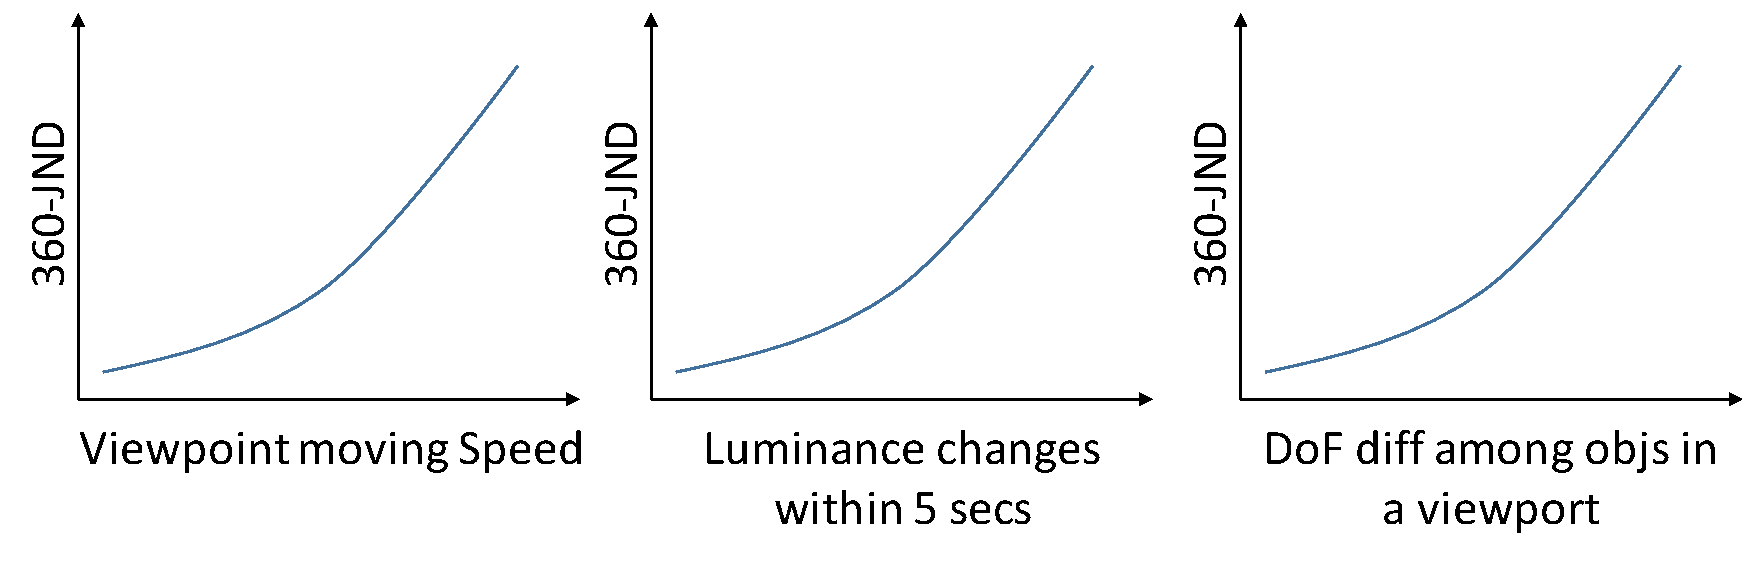
\includegraphics[width=0.5\textwidth]{figures/single-factor.pdf}
  \caption{Single-factor analysis. The impact of each of the three factors on \vrjnd.}
  \label{fig:single-factor}
 \end{figure}

\mypara{Impact of multiple factors}
\jc{briefly explain the impact of any two factors on \vrjnd, shown in Figure~\ref{fig:two-factor}. how does the graph show the correlations are mutually independent?}

\begin{figure}
  \centering
  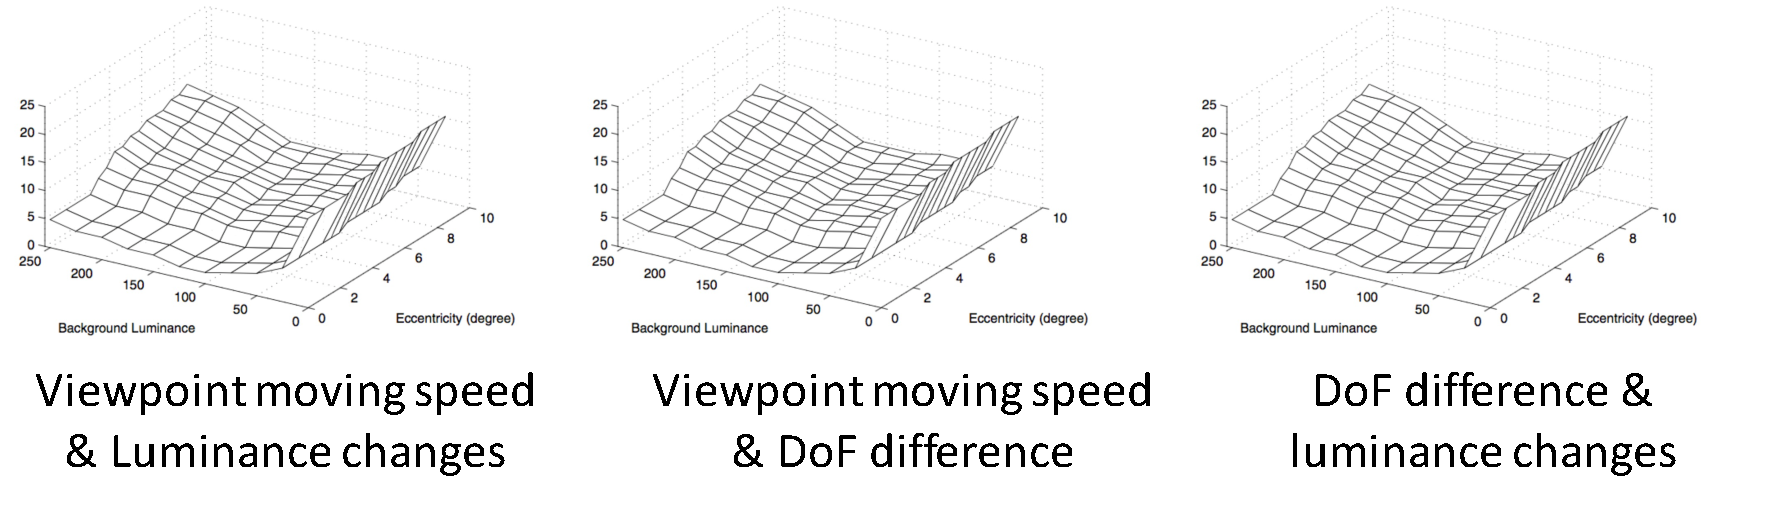
\includegraphics[width=0.5\textwidth]{figures/two-factor.pdf}
  \caption{Multi-factor analysis. The impact of two factors on \vrjnd appear to be largely mutually independent.}
  \label{fig:two-factor}
 \end{figure}

Lastly, this in no way provides a complete list of quality-determining factors. 
Rather, it provides a systematic methodology to incorporate future factors in the same framework of \vrvideo quality metrics.

%\begin{figure}
%  \centering
%  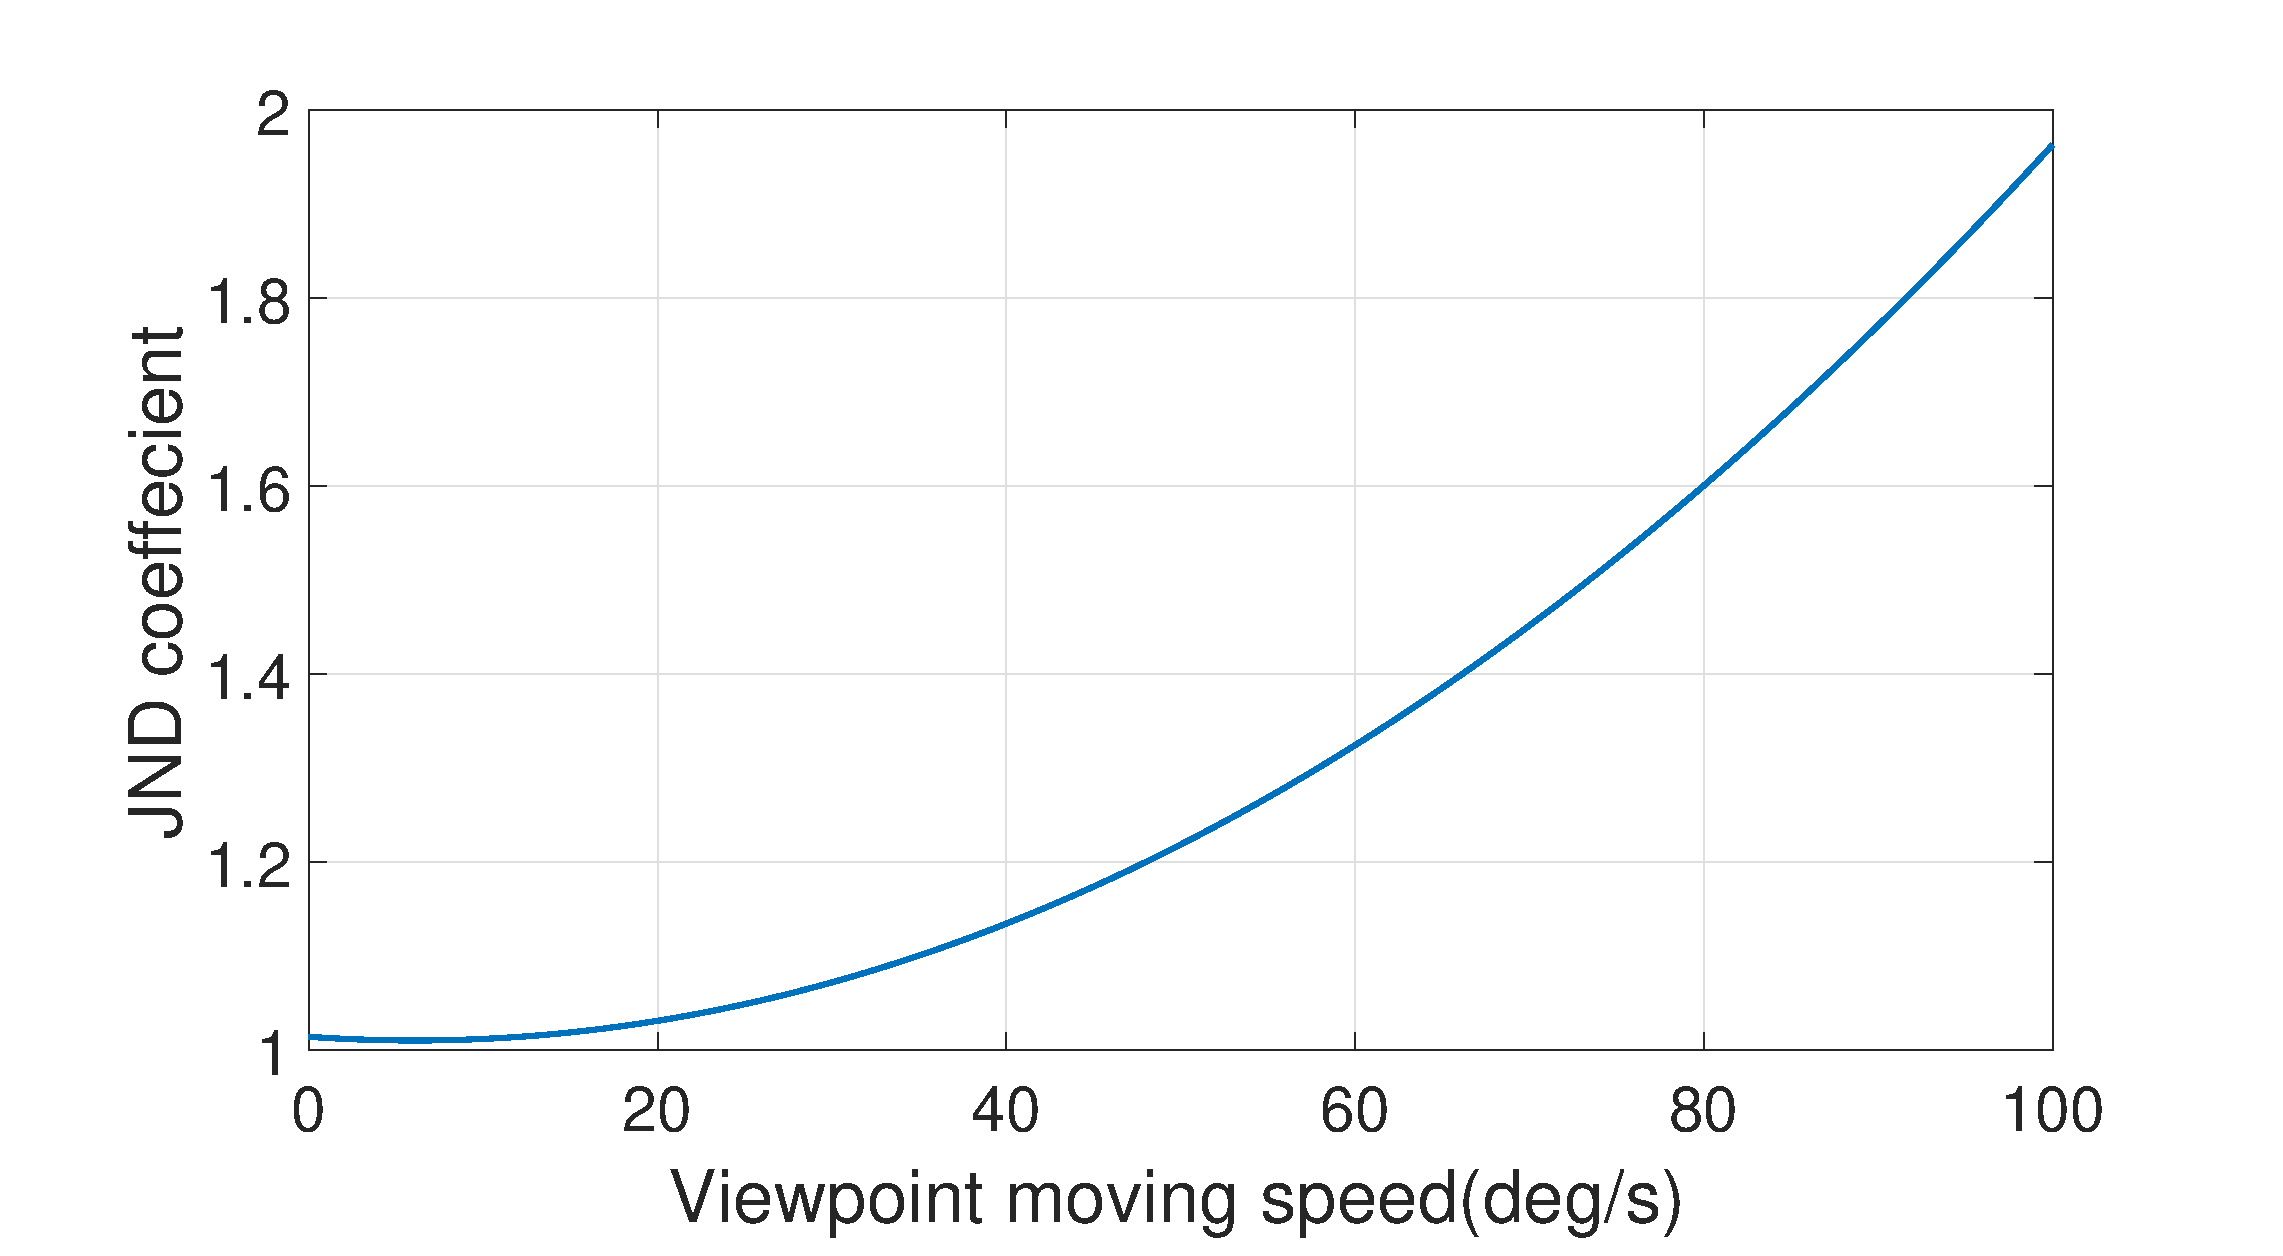
\includegraphics[width=2.5in]{images/JNDspeed.eps}
%  \caption{$f_{track}(v)$, the JND coefficient of viewpoint moving speed.}
%  \label{JNDspeed-track}
%  \end{figure}









\section{Object-based tiling scheme}

In this section we first introduce our object detection method. Based on this object detection, we describe our object-based tiling scheme and make comparison with state-of-art grid-like tiling schemes.

\subsection{Object Detection based on Quality-Bitrate Efficiency}

In the field of computer vision, there are many object detection algorithms which can cut a video into different content objects. However, in our video tiling scheme, the purpose of object  detection is little different. Actually we do not care if two adjacent tiles contain exactly the same object or they contain different objects. The most important thing is the probability of them to be allocated the same bitrate level by client. Even though two adjacent objects are different, if they have similar properties (like luminance, contrast, Depth of Field), we can also contain them in one tile because there is high probability for user to allocate them the same bitrate level.

To meet our purpose, for any rectangular tile which can be independently encoded, we define its \textbf{Quality-Bitrate Efficiency (QBE)} as follow:

\begin{alignat}{2}\
QBE = \frac{PSPNR_{highest} - PSPNR_{lowest}}{B_{highest} - B_{lowest}} \label{QBE}
\end{alignat}

where $PSPNR_{highest}$ / $PSPNR_{lowest}$ denotes the PSPNR value of this tile's highest / lowest bitrate version, and $B_{highest}$ / $B_{lowest}$ denotes the bitrate of this tile's highest / lowest bitrate version. In order to eliminate the influence for PSPNR by different user viewpoint positions, we only consider luminance, texture complexity and Depth-of-Field in QBE computation. These informations can be obtained completely on server-side.

In a video frame, different objects have different QBE. QBE is highly related to properties of content objects. According to PSPNR computation (Section 4), objects with very dark / light object luminance, complex texture or high depth of field, usually has higher QBE.

In perceived quality optimization, it is obvious that objects with high QBE is more likely to be allocated high bitrate (because it can improve more PSPNR in the same bandwidth cost), and objects with low QBE is more likely to be allocated low bitrate. So when two adjacent objects have similar QBE, they have high probability to be allocated the same bitrate level. 

\subsection{Tiling video by objects}

Based on above insights, we aim to cut the video into $T$ rectangular tiles of unequal size, such that content items within the same tile have similar QBE.

In this paper, tiling video by objects consists of 3 steps:

\textbf{Step 1: Partitioning the original video into 12*24 rectangular basic units of equal size.} 

Basic unit is the smallest unit of proposed object-based tiling. In the tiling process, each tile must be composed by one or several entire basic units which form a rectangular shape.

\textbf{Step 2: Computing QBE of each basic unit.}

We get QBE of each basic unit according to (\ref{QBE}). After that, suppose a tile $t$ consists of $N_t$ basic units $u_1$, $u_2$, ... , $u_{N_t}$ , we can compute its QBE Variance ($QBEV_t$) as follow:

\begin{alignat}{2}\
QBEV_t = \frac{\sum_{1 \le i \le N_{t}}{(QBE_{u_i} - E(QBE_{u_{i}}))^2}}{N_t}
\end{alignat}

where $E(QBE{u_i})$ is the average QBE of basic units in tile $t$:

\begin{alignat}{2}\
E(QBE_{u_i}) = \frac{\sum_{1 \le i \le N_{t}}{QBE_{u_i}}}{N_t}
\end{alignat}

A tile with high QBEV means visual properties (e.g. luminance, texture complexity) of objects in this tile have very different properties. A tile with low QBEV means objects in this tile are similar. So a good tiling scheme should keep each tile's QBEV value as low as possible.

\textbf{Step 3: Merging all basic units into T rectangular tiles, such that their weighted average QBEV is minimal.}

Suppose $V$ is the whole video frame. $R_i$ is the $i$th rectangular tile and $S_i$ is its area.This optimization problem can be formalized as following:

\begin{equation}
\begin{aligned}
\min \sum_{i = 1}^T QBEV_{i} S_i \hspace{3cm} \\
\text{s.t.} \bigcup _{i=1}^N R_{i} = V\hspace{3cm} \\
R_i \bigcap R_j = \emptyset \hspace{1cm} \forall 1 \le i, j \le T
\end{aligned}
\end{equation}

However, this optimization problem is a NP-hard problem, so we can not get the optimal solution in polynomial time. In practice, we apply a dynamic programming algorithm to get the suboptimal solution for this problem. In our implementation, we set $T = 72$ since it performs well in most situations.

\subsection{Comparison of object-based tiling and grid-like tiling}

We evaluate our tiling scheme and make comparison with traditional grid-like tiling schemes.

Fig. \ref{tiling} shows the PSPNR-bandwidth tradeoff of 3*6 grid tiling, 6*12 grid tiling, 12*24 grid tiling and proposed object-based tiling. 

  \begin{figure}
  \centering
  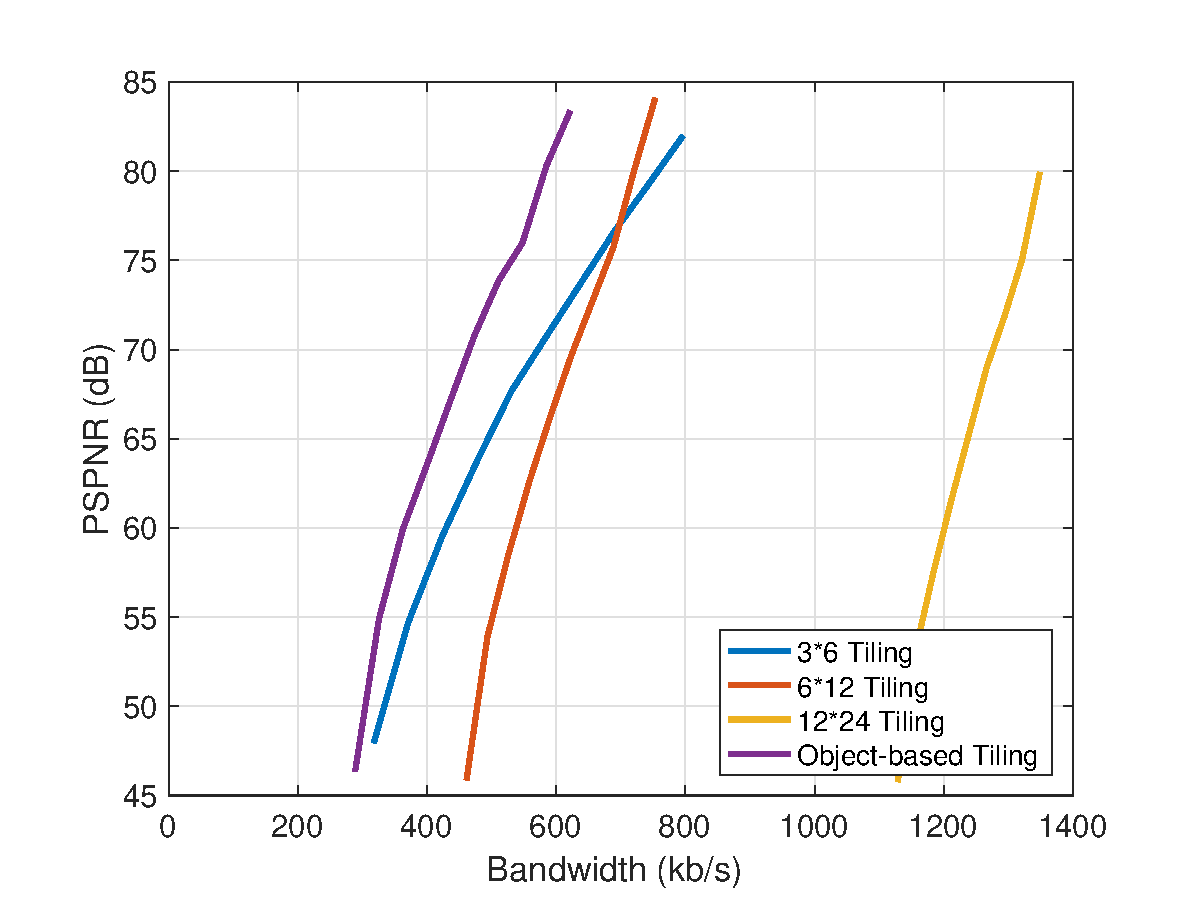
\includegraphics[width=2.5in]{images/tiling.eps}
  \caption{The PSPNR-bandwidth tradeoff of proposed Object-based Tiling scheme and traditional grid-like tiling scheme (3*6, 6*12 and 12*24).}
  \label{tiling}
  \end{figure}

For traditional gird-like tiling schemes, the performance of different tiling granularity depends on bandwidth. In low bandwidth, most part of video is allocated the lowest bitrate level. So there is no need to cut the video into many tiles. 3*6 tiling performs well because of its high bitrate efficiency. However, in high bandwidth, a coarse tiling granularity causes suboptimal bitrate allocation, so it is beaten by 6*12 tiling. Unfortunately, 12*24 tiling performs poorly in all bandwidth because of its serious bitrate efficiency problem.

Proposed object-based tiling scheme beats traditional grid-like tiling scheme of all bandwidth. In high bandwidth situation, it saves 20\% bandwidth compared with 6*12 grid-like tiling. Although 3*6 tiling's low bandwidth performance is near to proposed object-based tiling, its high bandwidth performance is far away from object-based tiling.


%!TEX root = main.tex

\section{Streaming protocol}
\label{sec:control}


Finally, we describe \name's streaming protocol. %, including its real-time quality adaptation algorithm that optimizes the user-perceived quality and how to implement it over existing DASH protocols. 
We focus on two questions: 
(1) how to adapt quality levels, spatially and temporally, to optimize the user-perceived quality in the presence of noises in user actions (\S\ref{subsec:adaptation}); and
(2) how to implement the \name adaptation logic over existing DASH protocols (\S\ref{subsec:compatible}).

\subsection{Robust quality adaptation}
\label{subsec:adaptation}
The \name adapts quality in two levels: {\em chunk-level} quality adaptation and {\em tile-level} quality adaptation. 
The chunk-level adaptation determines the total bitrate of the next chunk to meet buffer length target under the predicted bandwidth.
\name uses BOLA~\cite{bola}, one of the most popular bitrate adaptation algorithms, as the chunk-level adaptation. 

Within each chunk, the tile-level adaptation determines the quality level of each tile to maximize the perceived quality while ensuring the total size of the tiles does not exceed the bitrate of the chunk. 
Suppose the bitrate of a chunk $\Chunk$ is $\Bitrate_\Chunk$. The goal of the tile-level adaptation is to determine for each tile $\Tile\in\Chunk$ the quality level $\Quality_\Tile$, such that the total tile size of these tiles $\sum_{\Tile\in\Chunk}\Quality\leq \Bitrate_\Chunk$, and the total PSPNR $\sum_{\Tile\in\Chunk}\Area_\Tile\PSPNR_\Tile(\Quality_\Tile)$ is maximized. 
Here, the PSPNR of a tile $\Tile$ is weighted by its area $\Area_\Tile$.
Following the assumption that PSPNR is a linear function of quality level (\S\ref{sec:tiling}), we can rewrite the objective as max $\sum_{\Tile\in\Chunk}\Area_\Tile\Efficiency_\Tile\Quality_\Tile$, where $\Efficiency_\Tile$ is the efficiency score of tile $\Tile$. 
Although this is a linear optimization problem, its variable a discrete (quality level), which makes it a mix-integer programing problem. 
\name solves above problem with \fillme, an efficient approximation algorithm. \jc{Guan Yu: please briefly describe the solution}

It is important to notice that that formulation is sensitive to the accuracy of PSPNR, which depends heavily on the knowledge of user action, especially the three new quality-determining factors (\S\ref{sec:opportunities}).
Therefore, the tile-level adaptation seem very susciptible to the prediction errors of user actions, which are fundamentally difficult to predict accurately.

Suprisingly, however, one can achieve a reasonable robustness to the prediction errors of user actions with a simple prediction heuristics. 
The key insight is that although it is indeed hard to predict user actions accurately, it is possible to predict the {\em range} of user actions (\eg at least how fast the viewpoint will be in the next second). 
Figure~\ref{speed_analysis} shows an example of predicting the viewoint moving speed by \fillme. \jc{Guan Yu, what's the heuristics to predict the ``lower bound''?} 
Now, a reliable prediction on the lower bound of PSPNR of a tile is actually sufficient to determine the quality level of a tile because of the ``threshold'' effect of JND on PSPNR; \eg as long as the viewpoint moving speed is above some threshold, the difference between two quality levels would drop dramatically.

\begin{figure}
  \centering
  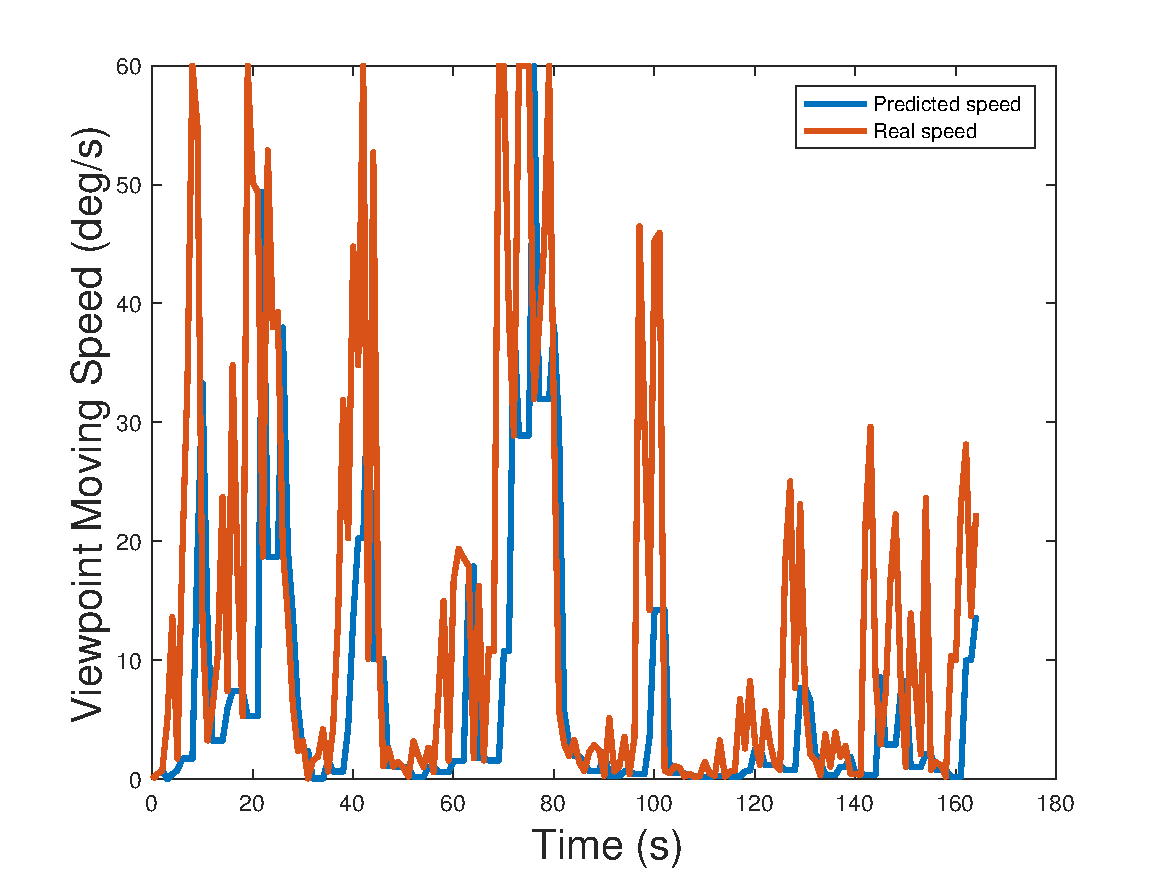
\includegraphics[width=2.5in, height=1in]{images/speed_analysis.pdf}
  \caption{An example of real viewpoint moving pattern and predicted viewpoint moving pattern.}
  \label{speed_analysis}
  \end{figure}


\subsection{DASH-compatible design}
\label{subsec:compatible}

While the logical workflow of \name is straightforward, it is nevertheless incompatible to the popular client-driven video streaming protocols.
\name bases its quality adaptation on the calculation of PSPNR (Equation~\ref{eq:pspnr}), which requires both user actions (for estimating JND) and the pixel-level information of the video. 
Because the pixel information is availale only at the video server, a straightforward implementation of \name would be to send the user action prediction (\eg how fast the viewpoint moves) to the server which than makes quality-adaptation decisions. 
This however violates a key tenet of the existing video streaming protocol that has spurred the wide popularity of \vrvideos---the server must be passive while the client makes the adaptation decisions. Otherwise, the servers would be specialized, rather than cheap web servers.

\begin{figure}
  \centering
  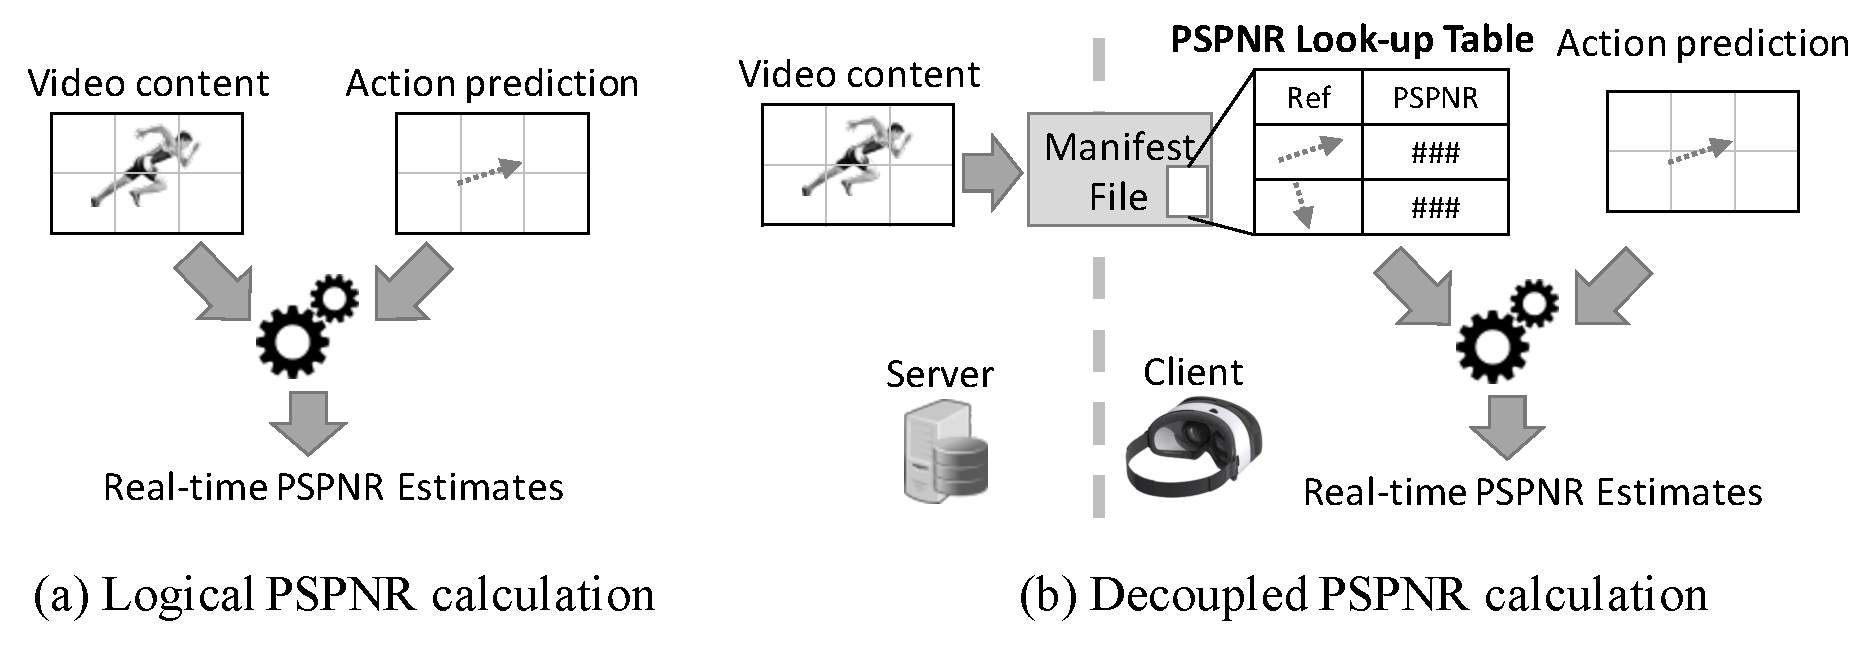
\includegraphics[width=0.5\textwidth]{figures/decoupling.pdf}
  \caption{Decoupling the logical PSPNR calculation workflow (a) into client and server by embededding the pre-computed PSPNR in the manifest file (b), so that the server is not longer involved in real-time PSPNR calculation or quality adaptation.}
  \label{fig:decoupling}
  \end{figure}


The idea behind \name is that one can decouple of calculation of PSPNR into an offline phase when the server pre-calculates the PSPNR for some ``representative'' user actions and stores them in a {\em PSNPR lookup table}, and an online phase when the client looks up the predicted user action in the table in real time. 
As illustrated in Figure~\ref{fig:decoupling}, this scheme is completely compatible with the existing client-driven video streaming protocol, like DASH: we can put the PSPNR lookup table in the manifest file (which will take no more than \fillme Bytes for a \fillme-minutes video), and the online PSPNR calculation and quality adaptation can be done purely on the client-side.

\section{Implementation}

%!TEX root = main.tex

\section{Evaluation}
\label{sec:eval}

We evaluate \name with both trace-driven simulation and real user survey. 
Our key findings are the following.

\begin{itemize}

\item \name achieves higher video quality and uses less bandwidth than state-of-the-art baseline across a wide range of video genres: \fillme\% higher quality (in both user rating and PSPNR) with the same bandwidth consumption, or \fillme\% less bandwidth consumption without drop in PSPNR.

\item \name is robust to errors in the prediction of viewer actions and available bandwidth. 

\item The offline tiling and online adaptation contributed substantial improvement to the overall gain of \name.

\item \name imposes only negligible overhead and actually reduce the client-side computing overhead.

\end{itemize}

\subsection{Methodology}

\mypara{Survey-based evaluation}
\jc{please fill in, no more than 1 para}

\mypara{Trace-driven simulation}
\jc{please fill in, no more than 1 para}

\mypara{Synthetic viewpoint trace generation}
\jc{please fill in, no more than 1 para}


\subsection{End-to-end improvement}

\mypara{User survey experiment}

\mypara{Large-scale trace-driven simulation}


\subsection{Robustness}

\mypara{Impact of bandwidth fluctuation}

\mypara{Impact of noises in viewpoint trajectory}


\subsection{System overhead}

\mypara{Client-side overhead}
\jc{cpu, ram, bandwidth}

\mypara{Server-side overhead}


\subsection{Component-wise analysis}




\section{Related work}
\label{sec:related}

\section{Discussion}

\jc{include the ethical discussion}

\jc{terms need to be cleared up: viewpoint vs viewport, quality vs QoE, velocity vs speed, DoV or FoV, etc}

\newpage
\jc{filling text to resolve vbox errors}



\bibliographystyle{ACM-Reference-Format}
\bibliography{reference}

\end{document}
